After implementing our tools, we conducted a user study with our tools. The goal of the study was to evaluate the suitability and quality of our tools. Thus, we designed multiple tasks that the participants had to complete with our tools. Because we need something to compare our results to, the participants also completed some tasks without our tools, using only the browser tools available in Google Chrome. In the following sections, we will describe the setup of the study, present our results and conclude with a discussion of our results.

\section{Setup}

The study was carried out in a room of the GlobIS group. The participants were sitting in front of a desktop PC with a 30-inch screen with a 2560x1600 resolution and had access to an English (US) keyboard and a mouse. The desktop PC was running Microsoft Windows 7 with Google Chrome Version 45. They also had access to two real devices: An Asus Nexus 7 (2012 version) Android tablet and an HTC M9 Android phone. Furthermore, they were given a tutorial sheet about JavaScript that contained some functions that are useful for DOM modification as well as arrays. Figure ~\ref{fig:study_setup} shows a picture of the setup of the study.

\begin{figure}[H]
  \centering
    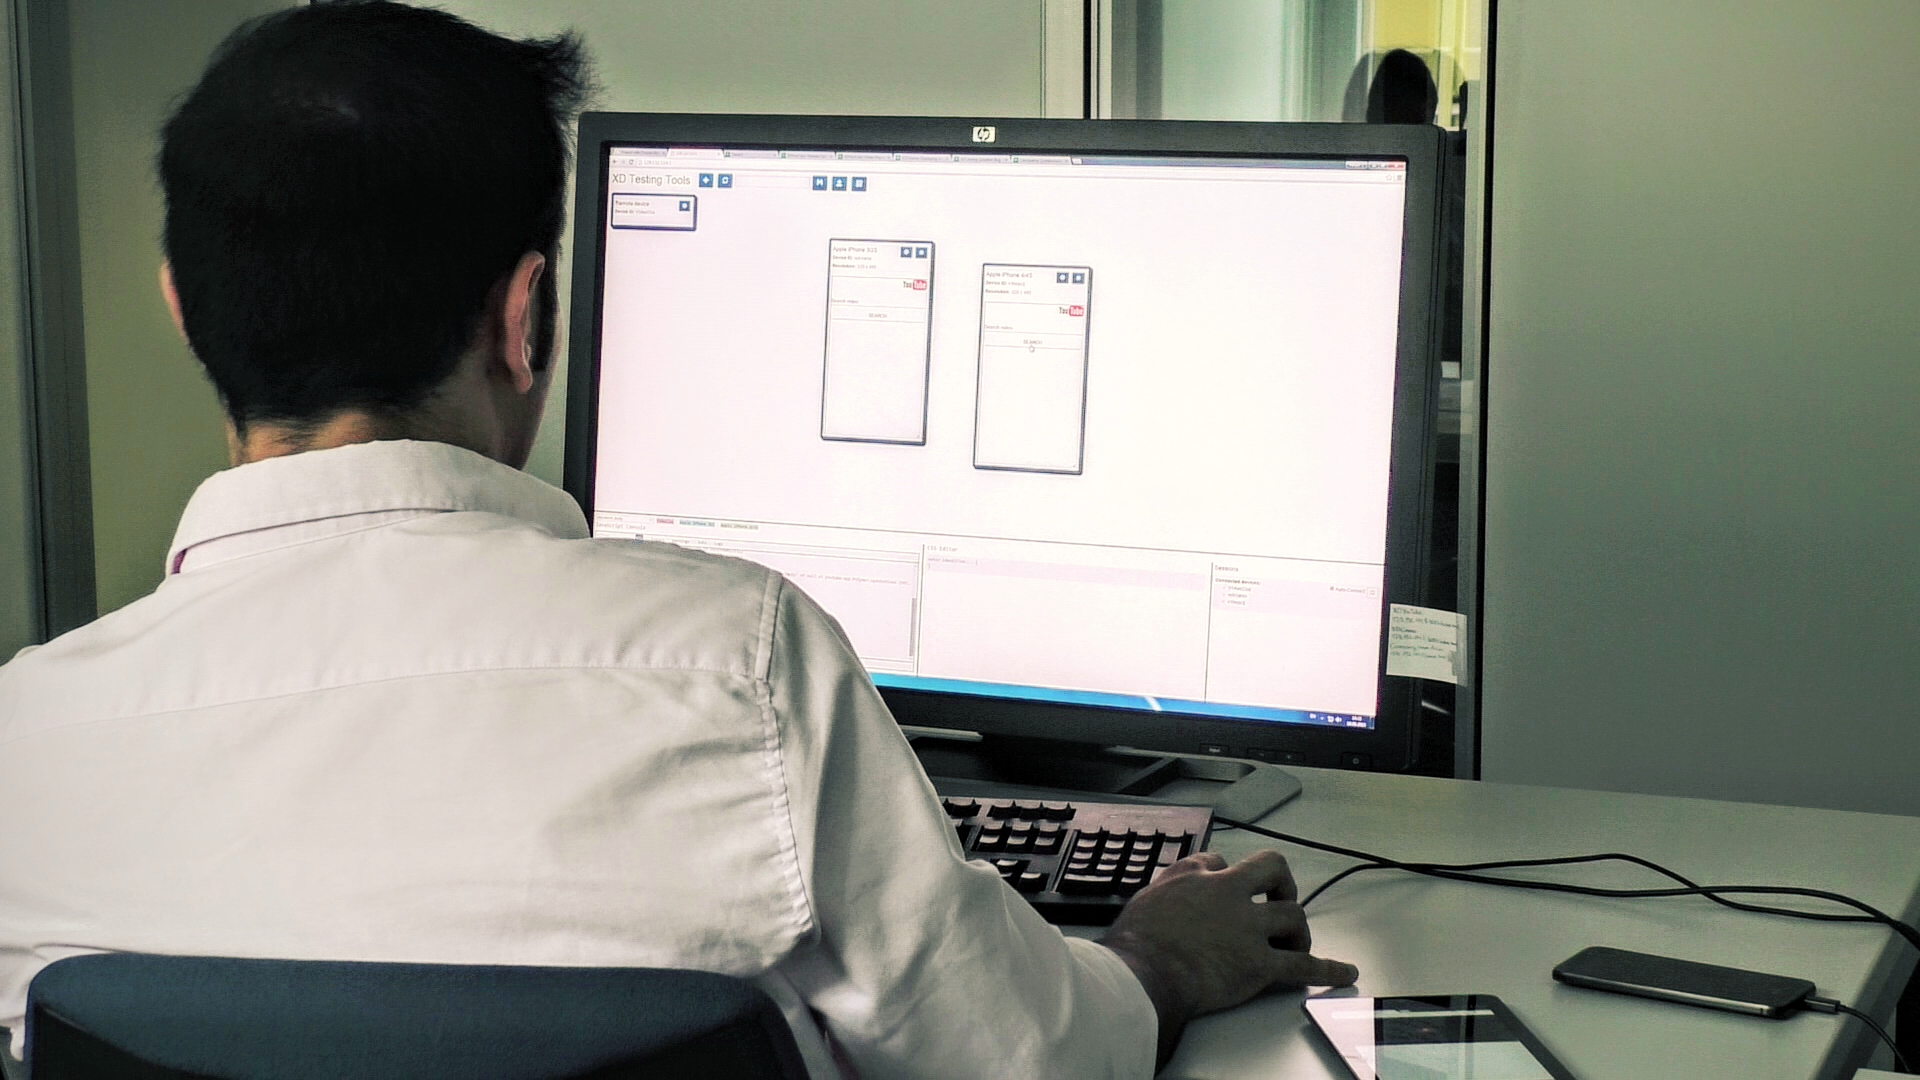
\includegraphics[width=0.8\textwidth]{images/study_setup2.png}
	\caption{Study Setup}
	\label{fig:study_setup}
\end{figure}

During the study, the instructor was sitting next to the participants and was available to answer any questions that occurred during the study. If a participant did not make any progress on a task for some time, the instructor also gave some hints to lead the participant in the right direction.

The participants had access to Chrome DevTools for all tasks. Furthermore, we set up multiple profiles on Chrome that the participants could use for emulating multiple devices. The participants could also remote debug the two real devices they had access to. The devices were already connected to the desktop PC by cable and the appropriate tab was already opened in the browser. Thus, the participants only had to navigate to the tab and click on inspect to remote debug a device. 

During the study, we disabled some features of our tools that were not required for completing the tasks so the participants would not be overwhelmed with the large amount of features that they had to learn how to use. We disabled the following features:
\begin{itemize}
	\item Changing the URL: The URL was given by the task anyway and it would have been of no use to change it during the study.
	\item Saving and loading device configurations: This feature is mainly useful for long-term use of our tools and is not needed for completing the tasks in the study.
	\item Record/Replay: We think that record/replay takes some time to get used to it and it is also only of limited use for simple tasks like the ones we used in the study. Furthermore, it might distract participants from the actual task because they might want to try it out even if it does not help them to complete the task.
	\item Inspecting HTML: The tasks in our study did not require modification or debugging of HTML, thus we deactivated this feature.
	\item Settings: The settings were disabled for the study because they were implicitly given by us.
\end{itemize}

All other features could be used by the participants. The following list provides an overview of the features the participants had access to:
\begin{itemize}
	\item Emulating devices
	\item Connecting real devices
	\item Connection features (auto-connect and drop-down list to connect to other devices)
	\item Shared JavaScript console
	\item Function debugging
	\item Shared CSS Editor
\end{itemize}
This list also represents the features that we want to evaluate during the study.

\subsection{Participants}

We recruited 12 participants that all were university members in the department of computer science at ETH Zurich. Most participants were either PhD or Master students, but there were also some Bachelor students. It was required that all participants have at least basic knowledge about front-end web technologies (i.e. HTML, CSS, JavaScript). However, the definition of "basic" was up to the participants and we did not ask participants to prove their experience before the study. Consequently, we also had some participants that had rather low experience with web technologies. We did not require participants to have any experience with cross-device application development as otherwise it would have been difficult to find enough participants. Nevertheless, two thirds of the participants actually did have some cross-device application development experience. The age of the participants ranged from 23 to 33 and the median age was 26. 

\subsubsection{Previous Experience}
We asked all participants about their previous experience with web application development and JavaScript in particular, as well as about their previous experience with responsive web applications and cross-device web applications. Furthermore, we asked them about whether they have used Chrome DevTools before and how they used them. The participants rated their skills in web application development and JavaScript on a 5-point Likert scale (see Figure ~\ref{fig:xp}) from basic to proficient and also gave the numbers of years in experience (see Figure ~\ref{fig:years_of_xp}) that they had in web application development and JavaScript.

\begin{figure}[H]
  \centering
    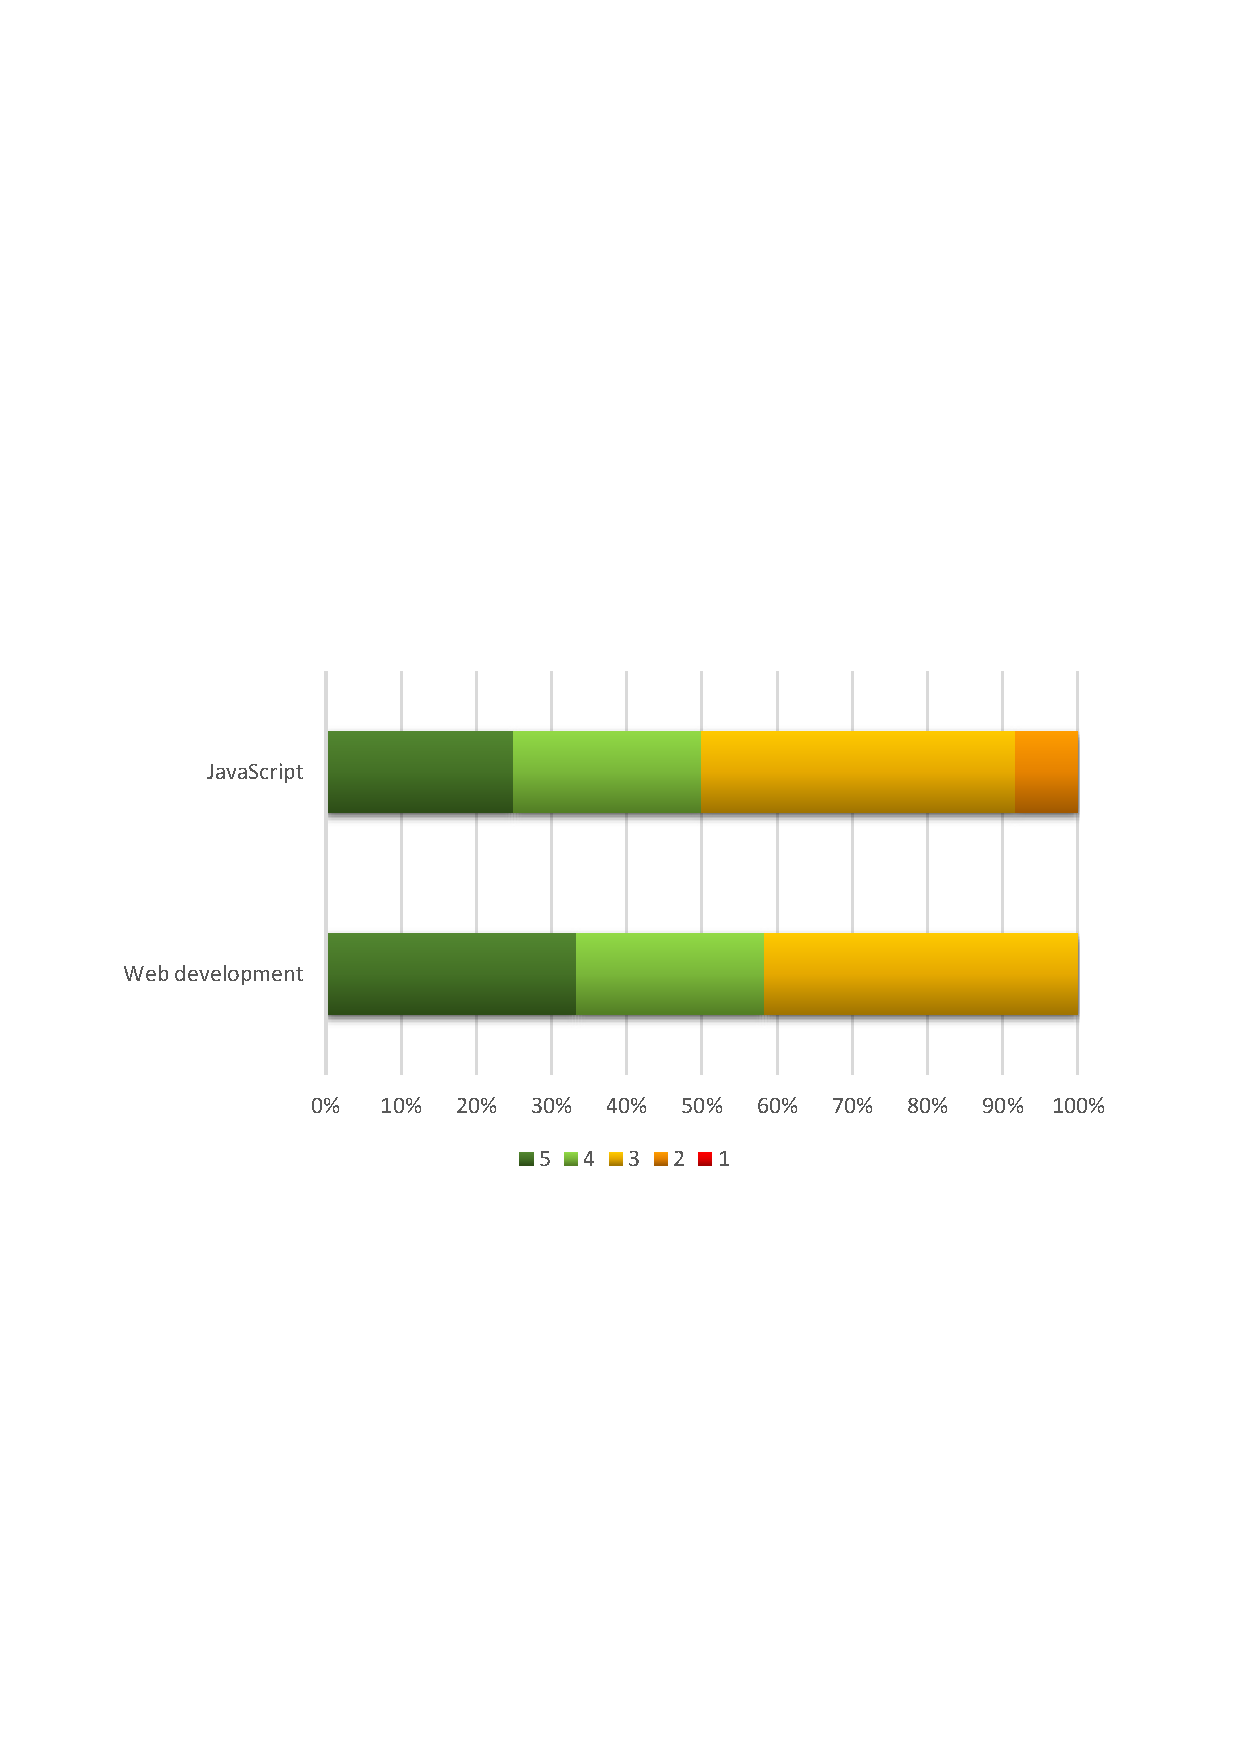
\includegraphics[width=0.8\textwidth]{images/charts/xp.pdf}
	\caption{Previous experience}
	\label{fig:xp}
\end{figure}

\begin{figure}[H]
  \centering
    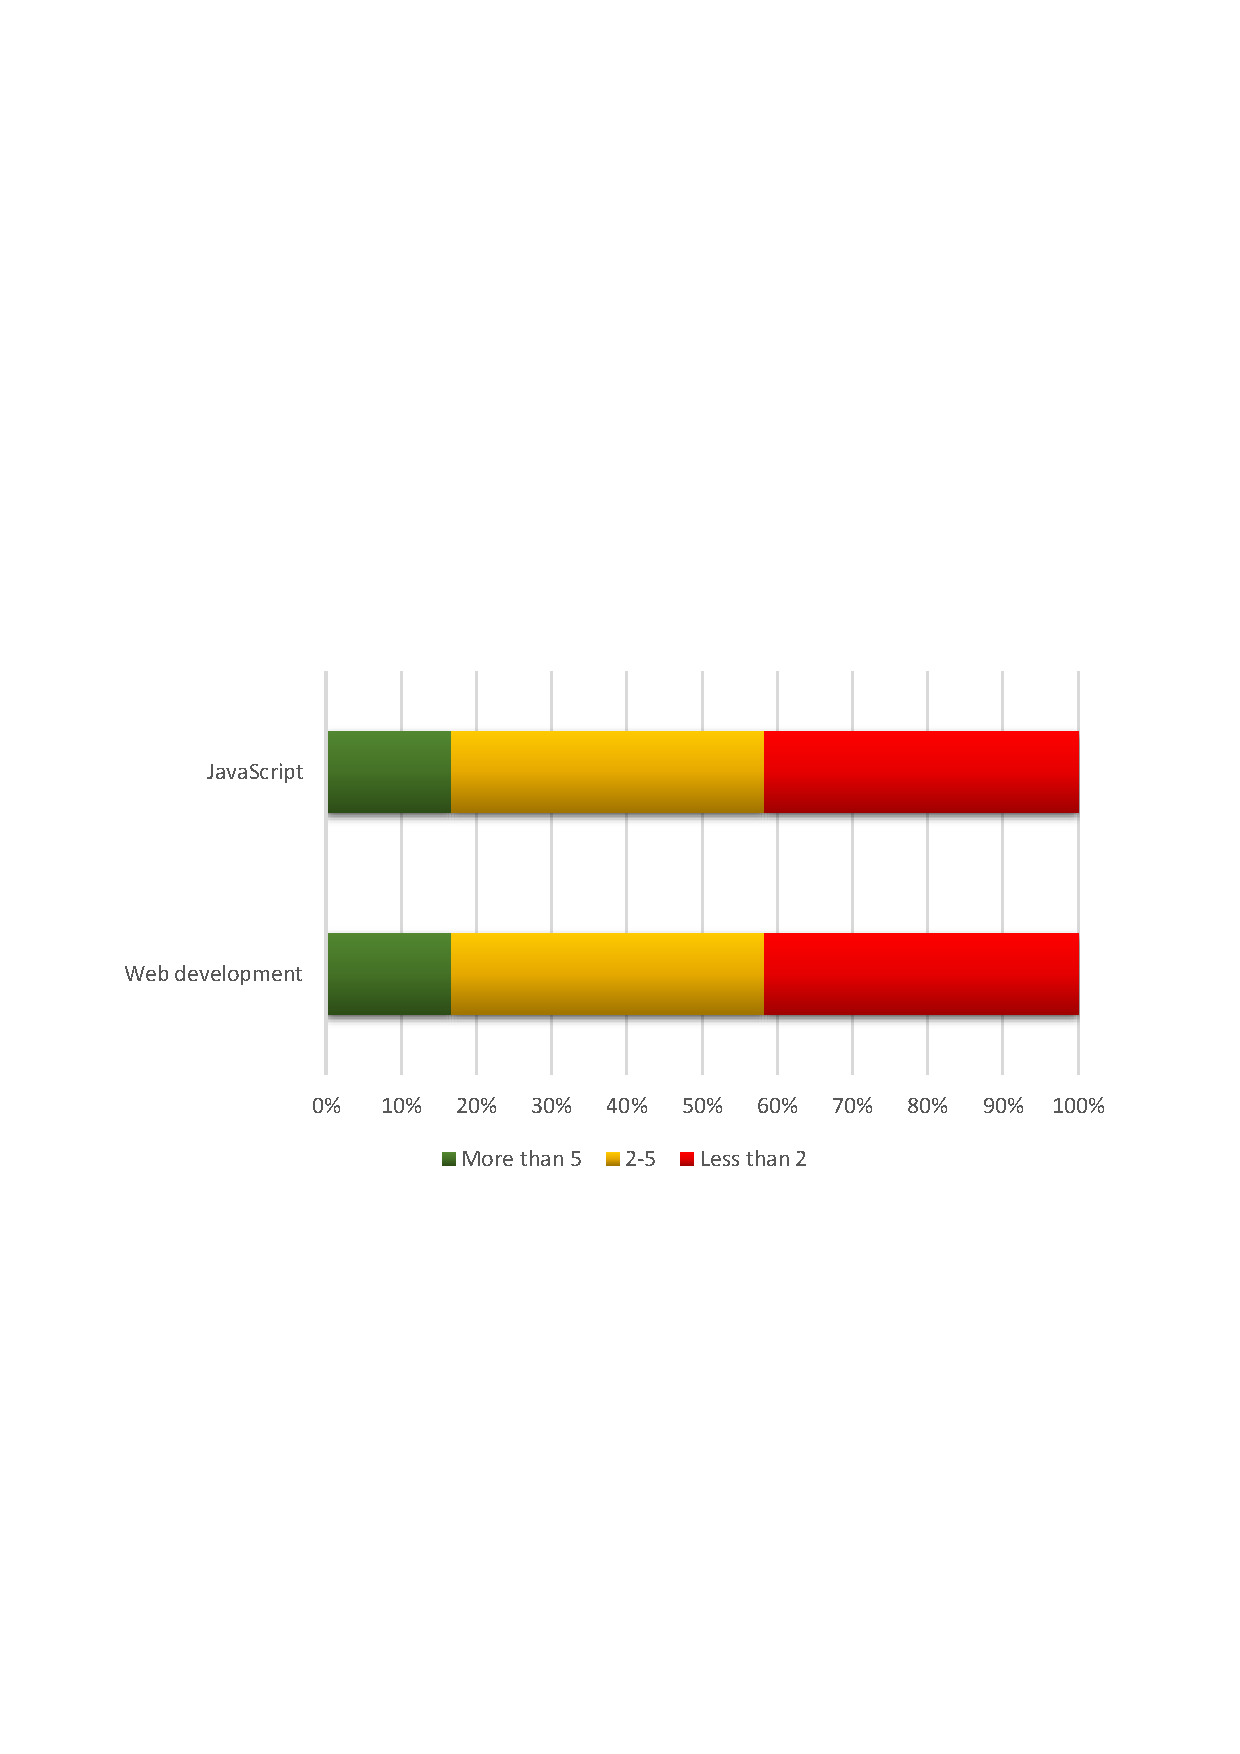
\includegraphics[width=0.8\textwidth]{images/charts/years_of_xp.pdf}
	\caption{Years of experience}
	\label{fig:years_of_xp}
\end{figure}

Nine out of the twelve participants stated that they already had some experience with developing responsive web applications. All except one used browser tools for emulating devices for testing their applications and all except two used real devices. Only one participant stated that they only used real devices for testing and no browser tools. One participant mentioned that they mainly re-sized browser windows to test their applications.

Eight participants already had some experience with cross-device application development. Again, most of them used browser tools for emulating devices and/or real devices for testing their applications. Four of them either used multiple browsers, multiple browser profiles or incognito modes to emulate multiple devices on one device. The fact that the other participants did not use any of those tools indicates that they probably used multiple devices at all times. This could either be because they do not know that they exist, because they are inconvenient or because they simply prefer real devices.

Most of the participants already had experience with Chrome DevTools, only two participants indicated that they had never used them before and one of them had used the developer tools of Firefox instead. We asked participants how often they used certain features of Chrome DevTools, in particular Device Mode, HTML and CSS inspection, JavaScript debugging and the console (see Figure ~\ref{fig:devtools_xp}). Not all participants had used Device Mode, which is no surprise, given that it is a rather new feature. All participants stated that they often use HTML and CSS inspection, thus this seems to be the most popular feature. The console was also used rather often. Surprisingly, JavaScript debugging was not that popular, less than half of the participants stated that they often use it.

\begin{figure}[H]
  \centering
    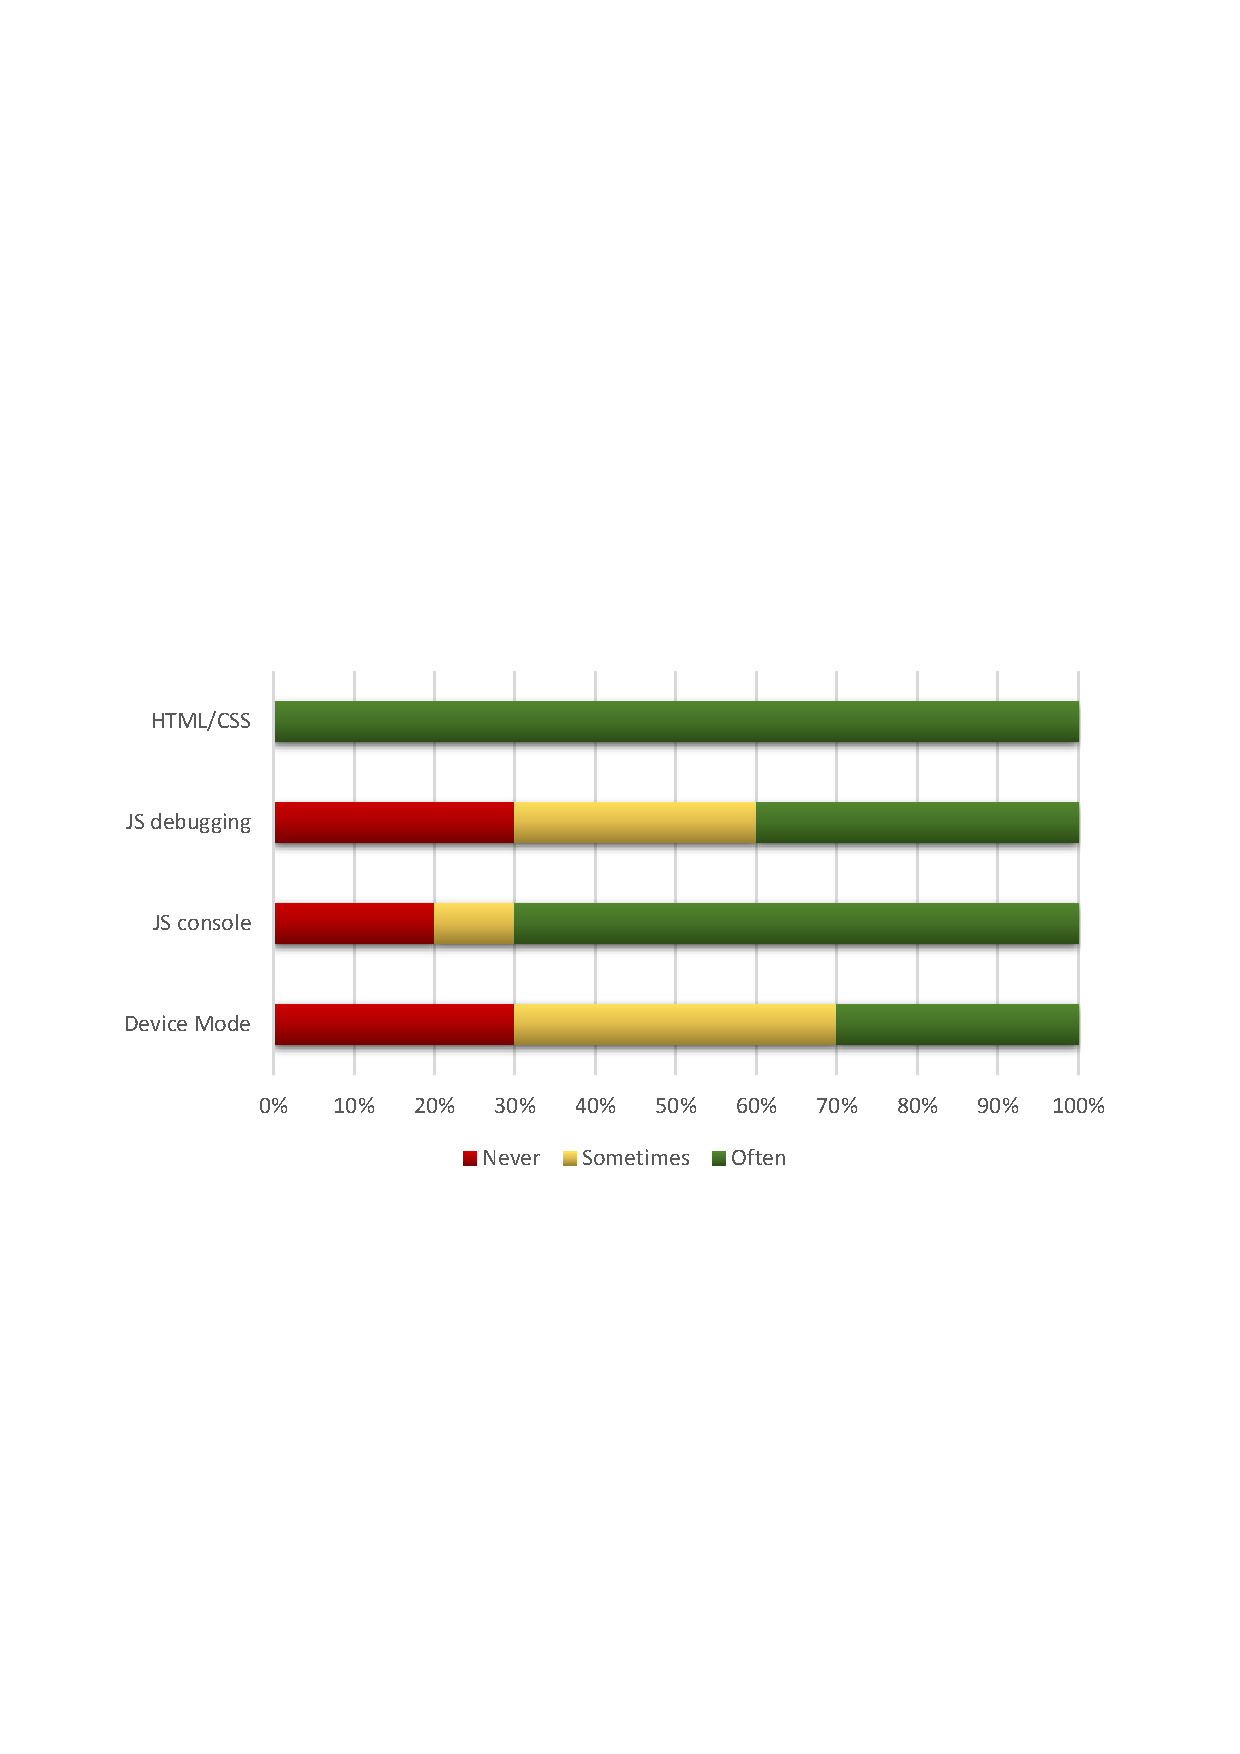
\includegraphics[width=0.8\textwidth]{images/charts/devtools_xp.pdf}
	\caption{Previous experience with Chrome DevTools}
	\label{fig:devtools_xp}
\end{figure}

\subsection{Tasks}

We used two different applications for the tasks, namely the two sample applications that we described earlier, XDCinema and XDYouTube. For each application, there were two tasks; one was about finding and fixing a bug in the code, and the other one was about implementing a new feature. The maximum time for the tasks where the participants fixed a bug was 15 minutes and the maximum time for implementing a feature was 30 minutes. After this time, we aborted the task unless it was clear that the participants would finish within the next 2 to 3 minutes. Each participant had to complete all four of the tasks; the tasks of one application with our tools, the tasks of the other application without them. The order of the applications as well as whether the first two tasks were with or without the tools was random. The participants completed the debugging task first and then the implementation task. Thus, the participants could learn how to use the application during the debugging task, which was considered easier than the implementation task, and were already familiar with the application for the second task.

\subsubsection{XDYouTube}
XDYouTube allows users to use their personal devices to search for videos and add them to a queue. The videos from the queue are then played one after the other on the largest of the devices. Users can also see the title and description of the currently playing video as well as the videos that are still in the queue by switching their device into landscape mode.

The first task with XDYouTube was to fix a bug concerning the video queue. As soon as one video finishes playing, the next video is dequeued from the queue and starts playing. However, when no video is in the queue, a JavaScript error occurs and causes the next video that is added to the queue not to play. The users were given a description of the task and then had to reproduce and fix it.  The participants were given a JavaScript file with two functions, one that adds a video to the queue and one that loads the next video at the end of a video.

For the second task, we asked participants to implement a remote control that can play and pause the current video from the controller devices. The participants had to implement two functions: One was called when the remote control button was clicked (the button as well as the event handler were already implemented), the other was called when a shared variable that states whether the video is paused or playing is changed. Thus, the participants had to change the shared variable whenever the button was clicked and to react accordingly on all devices if the shared variable changes, i.e. they had to pause or play the video on the device that plays the video and they had to change the text of the remote control button from "Pause" to "Play" and vice versa on all other devices. Furthermore, they had to change the CSS of the button such that it looked similar to a picture of a button that was given to them. The participants were given a JavaScript file with the two empty functions as well as a CSS file with the empty CSS selector of the button. Furthermore, they had access to a few helper functions:
\begin{itemize}
	\item pauseVideo(): Pauses the video
	\item unpauseVideo(): Unpauses the video
	\item isVideoPlaying(): Returns true if any video is currently active (even if it is paused)
	\item setPausedState(state): Sets the state of the shared variable
	\item getPausedState(): Returns the state of the shared variable (true if paused, false if playing)
	\item isPlayer(): Returns true if the device is responsible for playing the video and false if not
	\item isController(): Returns true if the device is responsible for controlling the video (add videos to queue, etc.) and false otherwise
\end{itemize}

\subsubsection{XDCinema}

XDCinema allows users to search for a city and date on one device. The device then shows a list of movies that play in this city on that date as well as the cinemas where the movie is played and the time that the movie starts. If the user clicks on a cinema, a summary of the movie as well as other information about the movie is shown on another device. If the user clicks on a cinema, the location of the cinema is shown on another device.

The first task was to fix a bug where the location of most cinemas was displayed wrongly, even though the information in the database is correct. The bug was that in one function, "j" was used instead of "i", which caused a wrong location to be returned. The participants were given a JavaScript file with a few functions related to getting and updating the location on all devices.

In the second task, the participants first had to complete the implementation of a function that shows the prices of each cinema where the movie plays below the description of the cinema. A skeleton for this function was already given where a loop over all cinemas that show the movie was already implemented, the participants only had to fill in the body of the loop. The second part of the task was to highlight the correct price (the participants were given a CSS class called "highlighted") when the user clicks on a cinema in the search view and to improve the CSS for highlighting. In the original version, highlighting used a light grey background color and a white text color which was not very readable. The participants were given a JavaScript file with the two functions as well as CSS file with the initial CSS of the "highlighted" class. The participants had access to the following helper function:
\begin{itemize}
	\item getCinemaPrice(cinemaName, city): Returns the price range of a cinema in a city
\end{itemize}

\subsection{Evaluation Methods}

In total, we used four different methods for evaluating the results of our user study. During the study, the participants had to fill out multiple questionnaires. Most our results are based on the questionnaires, the other methods for evaluation are only for clearing any inconsistencies, finding explanations for some things and maybe gathering some additional information that we missed during the study.

\subsubsection{Questionnaires}
At the beginning of the study, each participant had to fill out a questionnaire about their background information. The results of this questionnaire were already presented earlier. After each task, the participant had to fill out another questionnaire with the following questions:
\begin{itemize}
	\item It was easy to complete the task with the tools I had access to.
	\item I felt efficient completing the task with the tools I had access to.
	\item It was challenging to complete the task with the tools I had access to.
	\item The tools I had access to were well suited for completing the task.
\end{itemize}
The questions could be answered on a 5-level Likert scale from "Strongly Disagree" to "Strongly Agree". In the tasks where the participants had access to our tools, we also asked them to rate the usefulness of the individual features of our tools on a 5-level Likert scale. The following question was asked about the features: "How useful did you find the following features for completing the task?". The participants could answer this question for each feature on a 5-level Likert scale from "Not useful" to "Very useful". They could also choose the option "Not used" for features that they did not use while completing the task. For each task, there also was a comment field where the user could write down any additional comments that they had about the task or the tools they had access to.

After completing all tasks, the participants had to fill out a final questionnaire where they could answer some questions that compare our tools to the usual Chrome browser tools. They had to answer the following questions:
\begin{itemize}
	\item Did you find it easier to debug with or without the tool?
	\item Did you feel more efficient debugging with or without the tool?
	\item Did you prefer debugging with or without the tool?
	\item Did you find it easier to implement a feature with or without the tool?
	\item Did you feel more efficient implementing a feature with or without the tool?
	\item Did you prefer implementing a feature with or without the tool?
\end{itemize}
For those questions, the participants could either say that they preferred our tool, the normal browser tools, or that they did not have a preference.

In addition, they also answered some general questions about our tool.
\begin{itemize}
	\item It was easy to learn how to use the tool.
	\item I felt confident using the tool.
	\item The tool was unnecessarily complex.
	\item The tool would be useful for debugging cross-device applications.
	\item The tool would be useful for implementing cross-device applications.
	\item I would use the tool for debugging cross-device applications.
	\item I would use the tool for implementing cross-device applications.
\end{itemize}
Those questions could again be answered on a 5-level Likert scale from "Strongly Disagree" to "Strongly Agree".

Finally, the participants could state which features of the tool they would use for debugging and implementing cross-device applications and they could also write some comments about the tool if they wanted to.

\subsubsection{Video Recording}
In addition to letting participants fill out questionnaires, we also used a video camera to record the participants while completing the tasks. This was mainly done to make sure that no important information was lost and so some strategies for solving tasks could be extracted from the videos. 

\subsubsection{Personal Feedback}
At the end of the study, participants were encouraged to share any comments that they still wanted to mention and to give their opinion about the tool. Any comments that the participants had given during the study were also noted.

\subsubsection{Time Measuring}
For each participant, the time required for completing each task was measured. This was mainly done to detect any major discrepancies between completion times with and without the tool. However, exact times are not considered relevant for evaluation because they highly depend on the participant and on the hints given by the instructor during the study.

\section{Results}

In the following sections, we will first present the results from the individual tasks and then the more general results. For each task, we will compare how people answered the questions in the per-task questionnaires with and without our tools. 

\subsection{XDCinema: Fixing a Bug}

The results for the task where the participants had to fix a bug in XDCinema can be seen in Figure ~\ref{fig:xdc_bug_comparison}. The figure shows the median values for the questions asked after the task with and without our tools. For the question that asks about how challenging it was to complete the task with the tools the participant had access to, a lower value is better; for all other questions, a higher value is considered better. There is a rather big difference in the median value for the suitability of the tools, while the differences are smaller for the other questions. The participants felt only slightly more efficient when completing the task with our tools and considered the task as slightly less challenging. In the question about the easiness of the task, exactly the same median value can be observed both with and without our tools. One reason for the bigger difference in the suitability could be that unlike easiness and efficiency, suitability does not really depend on the task itself. In other words, if a task is difficult, the easiness will be rated lower regardless of whether our tools are used or not and if a task is time-consuming, the efficiency will be rated lower. On the other hand, the suitability of the tools for the task does not change with the difficulty or duration of the task. However, it would still be desirable that our tools make debugging cross-device applications easier and more efficient instead of just being more suited. For this task, it seems that our tools mainly made the task more enjoyable, but did not have any other effects. This could also be due to the fact that the bug is rather trivial and debugging does not necessarily help much anyway.

\begin{figure}[H]
  \centering
    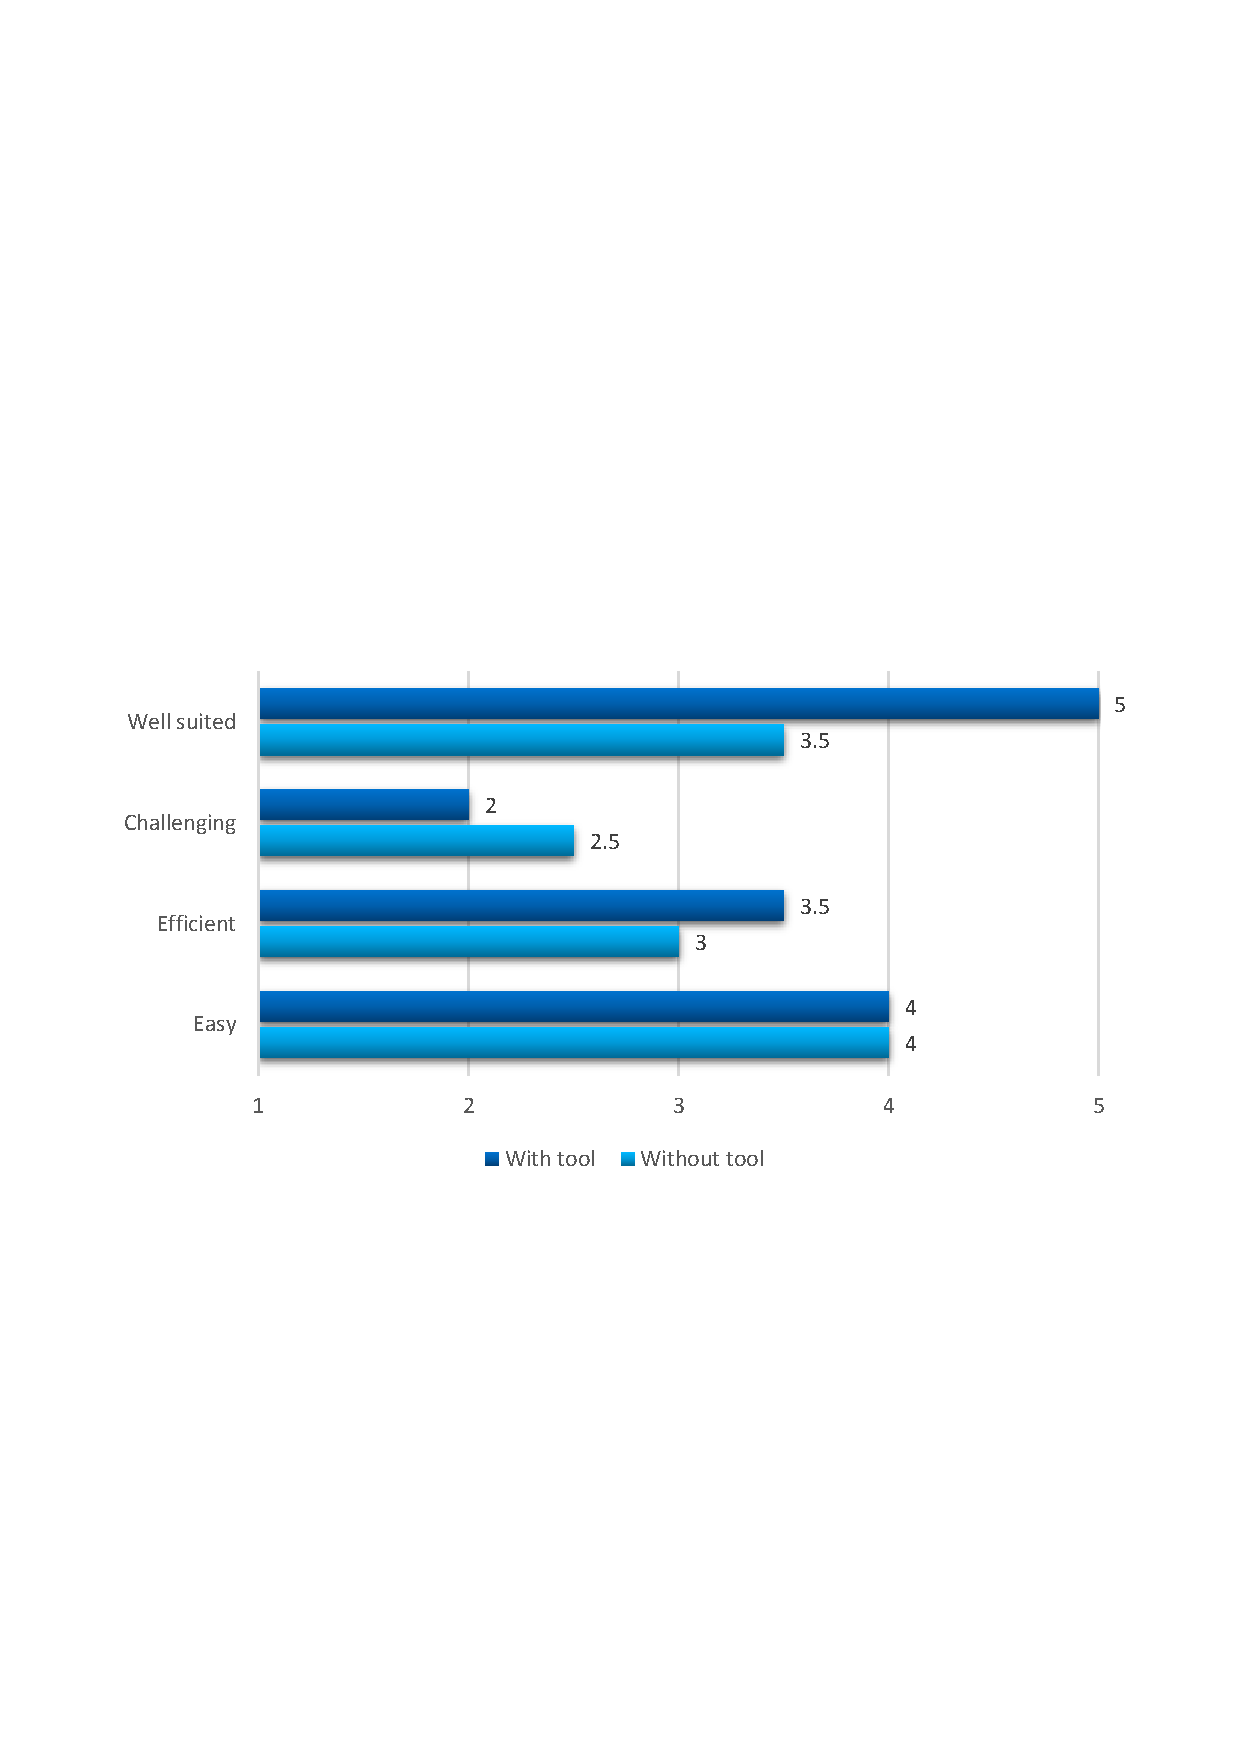
\includegraphics[width=0.8\textwidth]{images/charts/xdc_bug_comparison.pdf}
	\caption{XDCinema debugging task - Comparison}
	\label{fig:xdc_bug_comparison}
\end{figure}

Figure ~\ref{fig:xdc_bug_features_used} shows how many participants used the individual features of our tools and how useful they found them. Obviously, the figure only includes the participants that had access to our tools. None of the participants used real devices and all of them used device emulation instead. However, two participants rated device emulation with a 3, which indicates that they found it somewhat useful for the task, but not extremely useful. This could again be due to the fact that the bug they had to fix is actually rather trivial and could maybe even be solved faster by just looking at the code. The connection features and function debugging were used by all except one participant and were very appreciated by the participants. The shared JavaScript console was rather unpopular for this task, probably also due to the simplicity of the task and due to the fact that the bug produced no JavaScript errors that would be displayed in the console.

\begin{figure}[H]
  \centering
    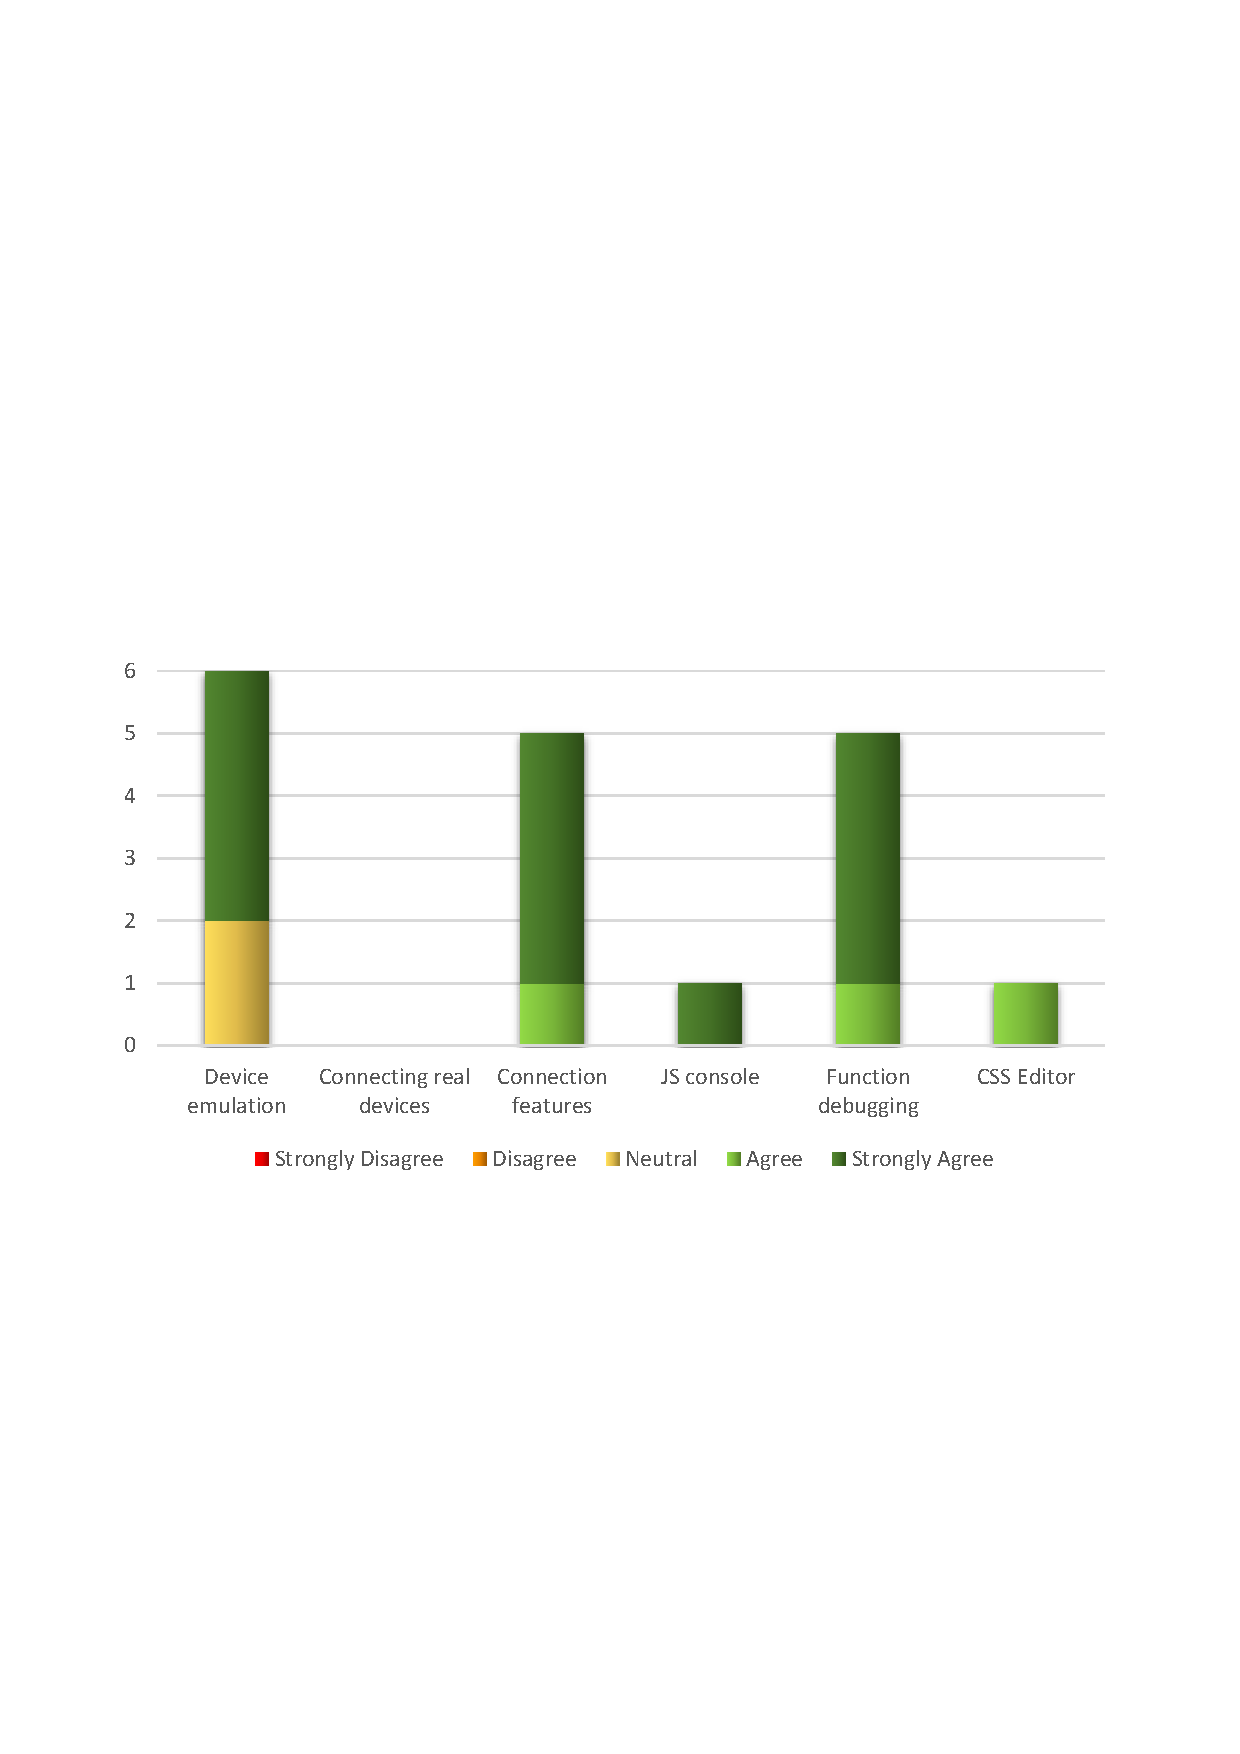
\includegraphics[width=0.8\textwidth]{images/charts/xdc_bug_features_used.pdf}
	\caption{XDCinema debugging task - Features used}
	\label{fig:xdc_bug_features_used}
\end{figure}

\subsection{XDCinema: Implementing a Feature}

In Figure ~\ref{fig:xdc_impl_comparison}, the results for the implementation task in XDCinema can be seen. Again, the figure shows the median values. In this task, the difference in suitability is less pronounced than in the XDCinema debugging task, but the difference for the question about efficiency and easiness is larger. In general, the task was considered as rather easy independent of the tools the participant had access to, although participants that had access to the tools perceived it as even easier. The median value of five with our tools suggests that participants had no problems completing the task at all when they had access to our tools. Similar results can be observed concerning efficiency. The difference in median values suggests that the participants felt quite a bit more efficient with our tools. Surprisingly, if we compare the average and median completion times for this task, the participants that had access to our tools were considerably slower (comparing median values, the participants that had access to our tools were about 9 minutes slower). In fact, this is the only task where the difference in completion times with and without our tools is noticeable; the completion times for all other tasks are almost equivalent. However, those two facts do not necessarily contradict each other, as there were participants with very different experience levels and as it is random which participants have access to our tools and which not and the number of participants is rather low, it is possible that almost all participants with low experience fall into the same category. In general, the completion times should not be considered as especially relevant, after all the instructor also gave some hints during the study and this can also distort completion times significantly. However, it would be interesting to see how completion times differ if there is a larger number of participants. 

\begin{figure}[H]
  \centering
    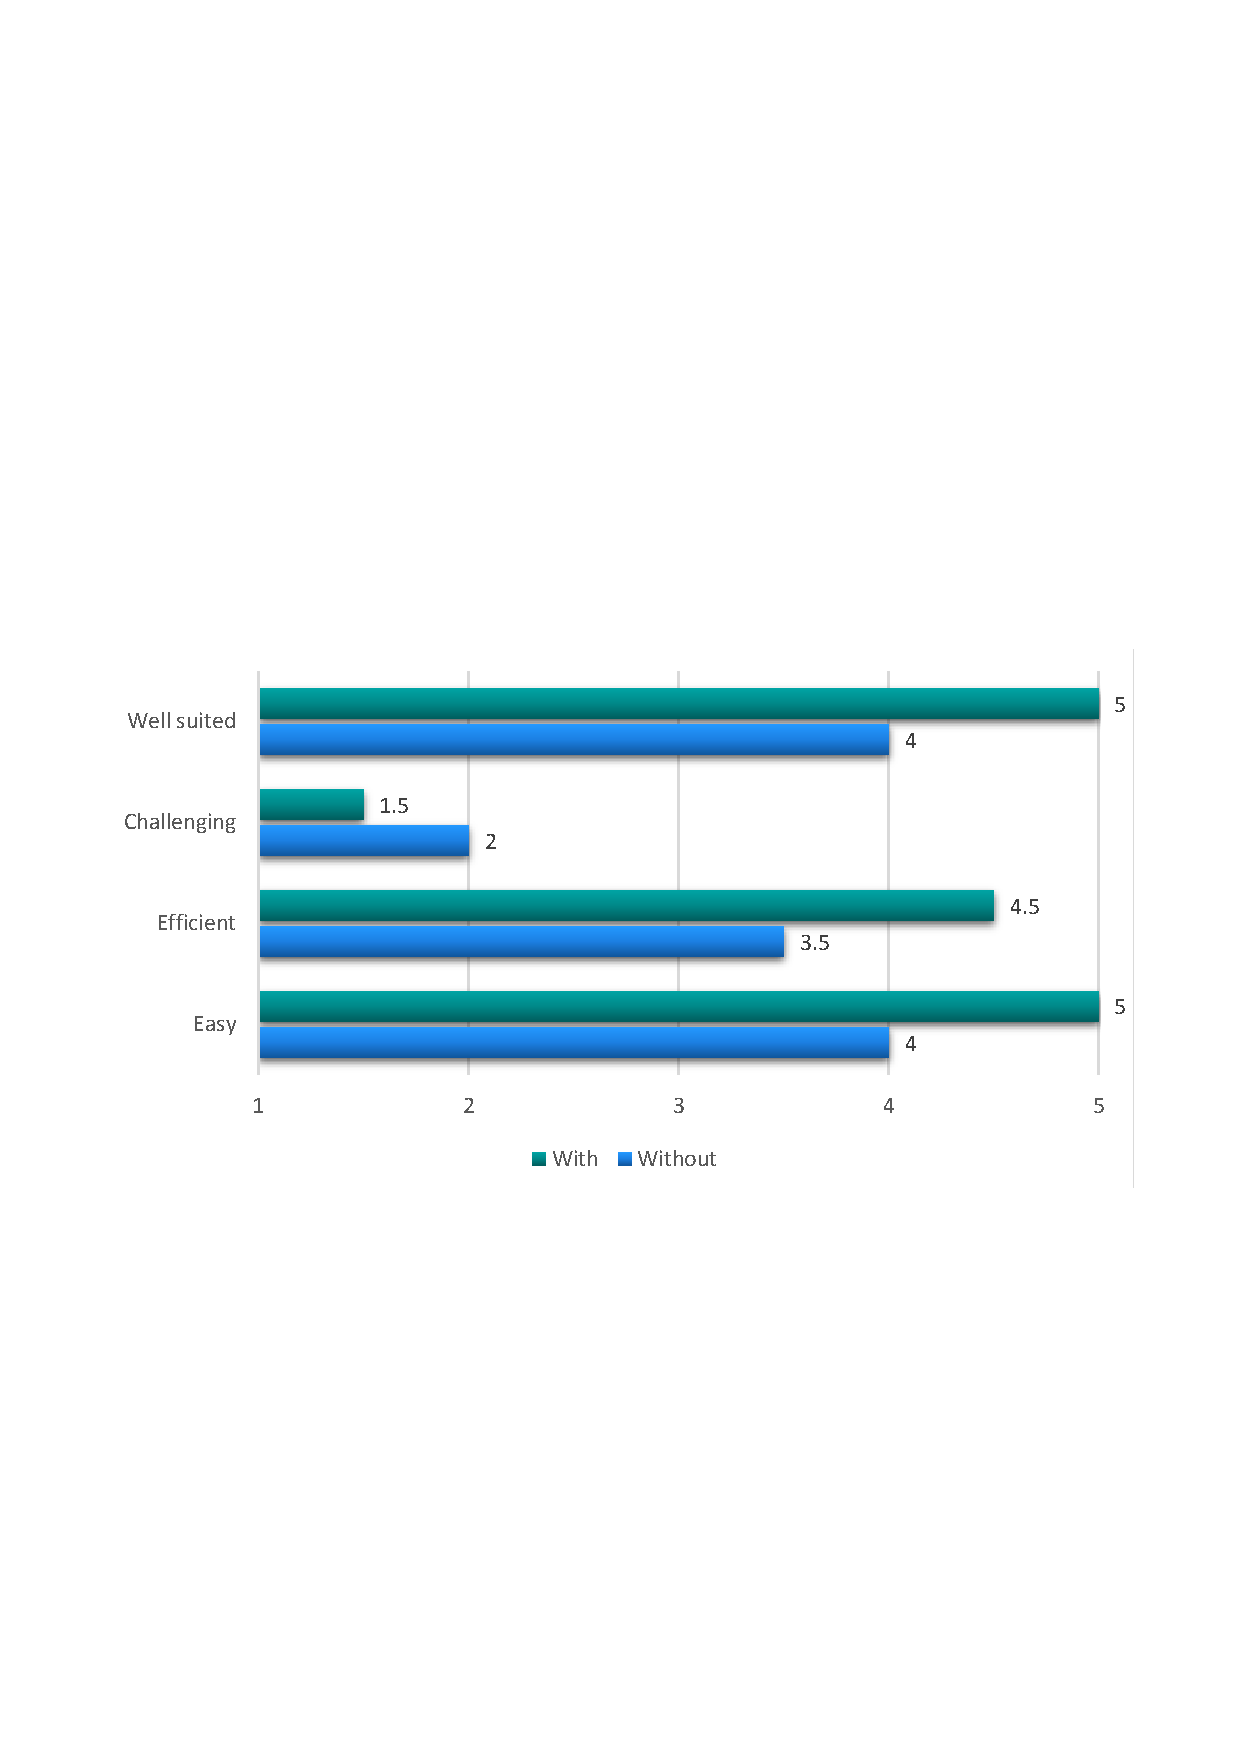
\includegraphics[width=0.8\textwidth]{images/charts/xdc_impl_comparison.pdf}
	\caption{XDCinema implementation task - Comparison}
	\label{fig:xdc_impl_comparison}
\end{figure}

Figure ~\ref{fig:xdc_impl_features_used} again shows the use and the ratings of the individual features. Again, no participant used the real devices. All participants used device emulation and the connection features and in contrast to the debugging task in XDCinema, device emulation was rated as very useful by all participants. Function debugging was used a bit less than in the debugging task, but the shared JavaScript console was used much more. It makes sense that function debugging is used more when fixing a bug; if one implements a feature and it works immediately when testing it, there is no need to debug a function, but if one has to fix a bug, there obviously must be a bug in a function and thus it makes much more sense to debug functions. The shared JavaScript console was rarely used to send commands and most participants did not use logging for solving the task, but many participants had some syntax errors when first testing the feature and noticed the error messages in the console. This also explains why the console was used more in the implementation task than in the debugging task: Generally, console outputs are very useful for debugging, but in this specific bug, there were no errors in the console in contrast to the implementation task, where syntax errors were shown in the console. Finally, the CSS editor was also used by some participants in this task. However, some completed the CSS part of the task using only the CSS file. This may be because they did not think of the CSS editor at this specific moment, or because they know CSS so well that they can just write everything down immediately, or also because they do not consider the CSS editor useful for this task.

\begin{figure}[H]
  \centering
    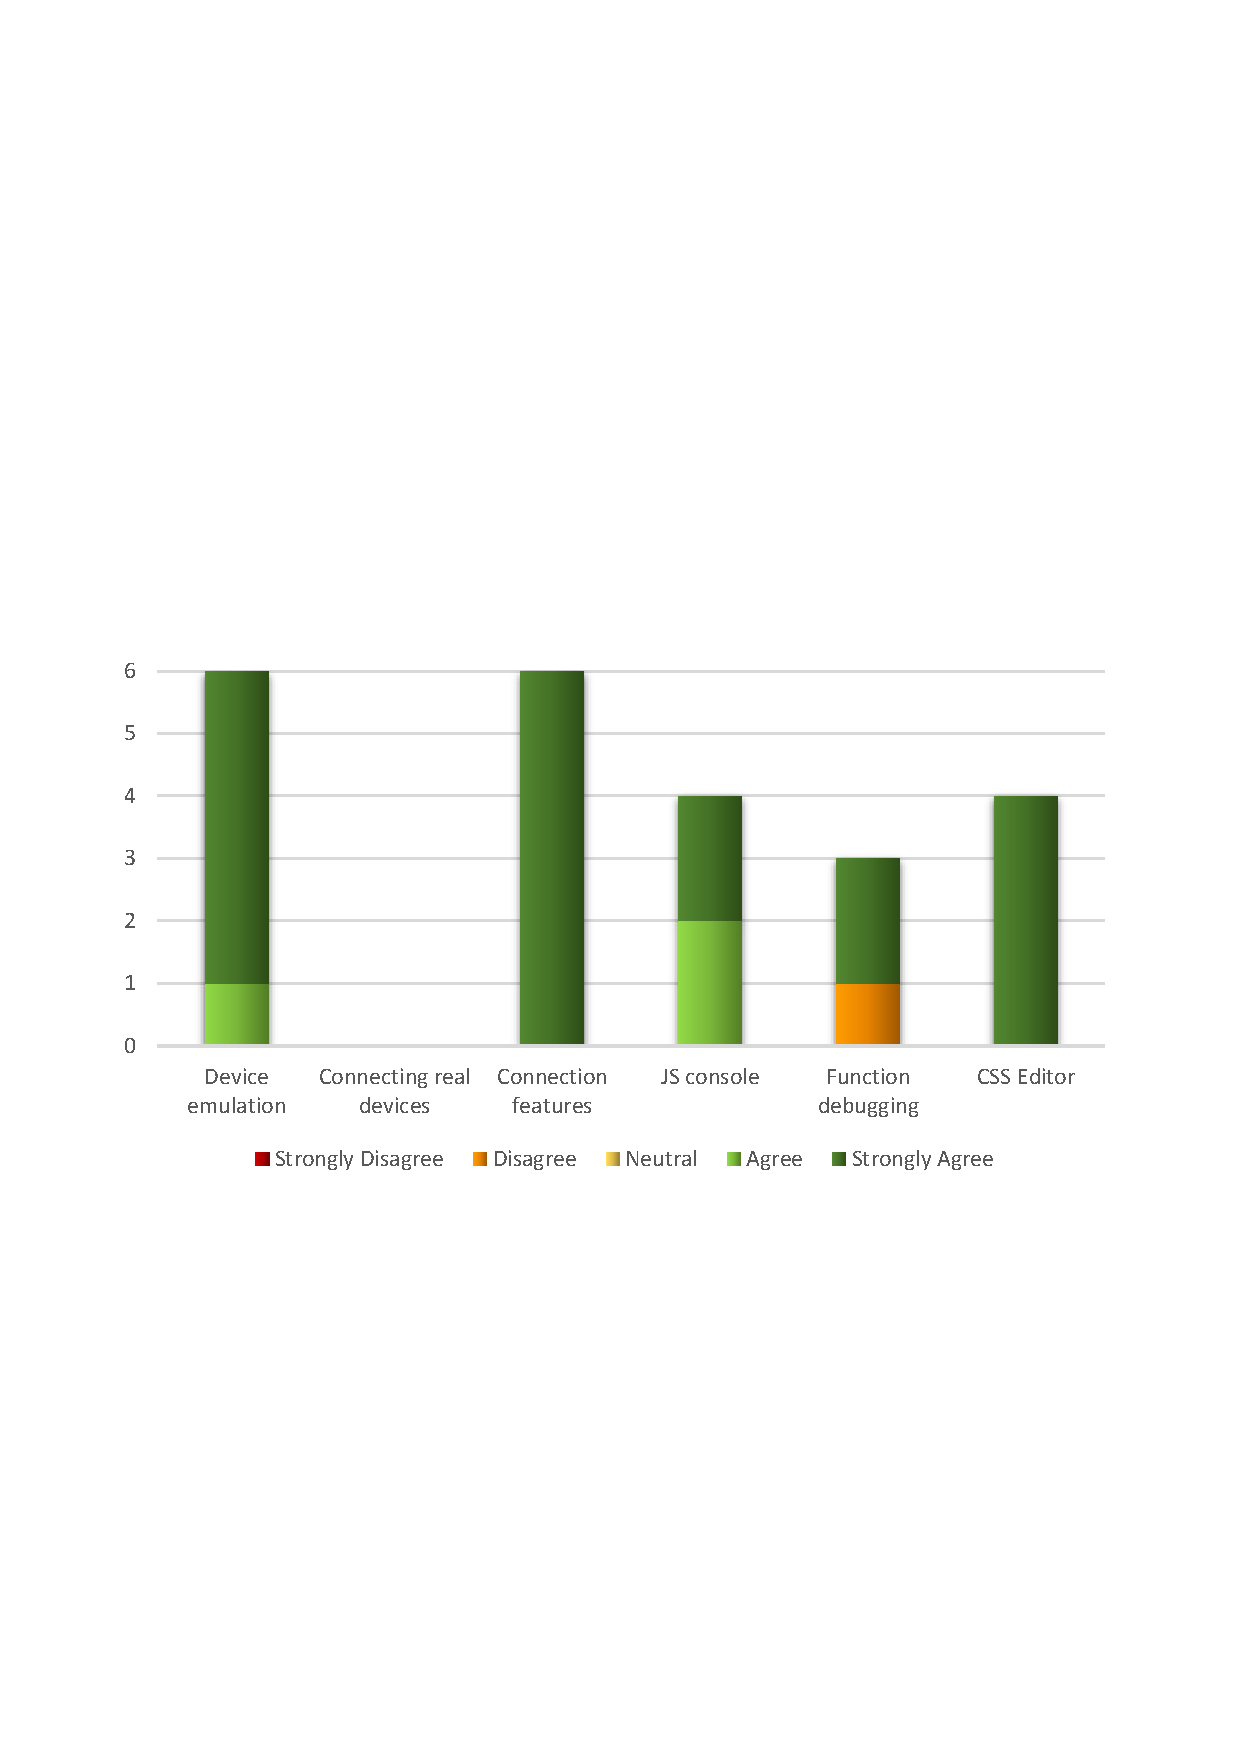
\includegraphics[width=0.8\textwidth]{images/charts/xdc_impl_features_used.pdf}
	\caption{XDCinema implementation task - Features used}
	\label{fig:xdc_impl_features_used}
\end{figure}

\subsection{XDYouTube: Fixing a Bug}

Figure ~\ref{fig:xdyt_bug_comparison} shows the results for the debugging task in XDYouTube. The difference in suitability between our tools and the usual browser tools was most significant in this task with a difference of 2. The difference in efficiency is also rather large. Surprisingly, the task was rated as almost equally easy and challenging with and without our tools despite the large differences in the other questions. It seems that for this task, our tools did not make the task any easier to solve, but the participants felt more efficient when completing it. During the study, we noticed that most participants had problems reproducing the bug and almost all participants required some hints and finished the task more or less around the time limit. This could explain why the task was perceived as equally difficult with and without our tools: The participants did not really find the bug without help anyway, independent of whether they had access to our tools, so it makes sense that they would consider the task as difficult in general. 

\begin{figure}[H]
  \centering
    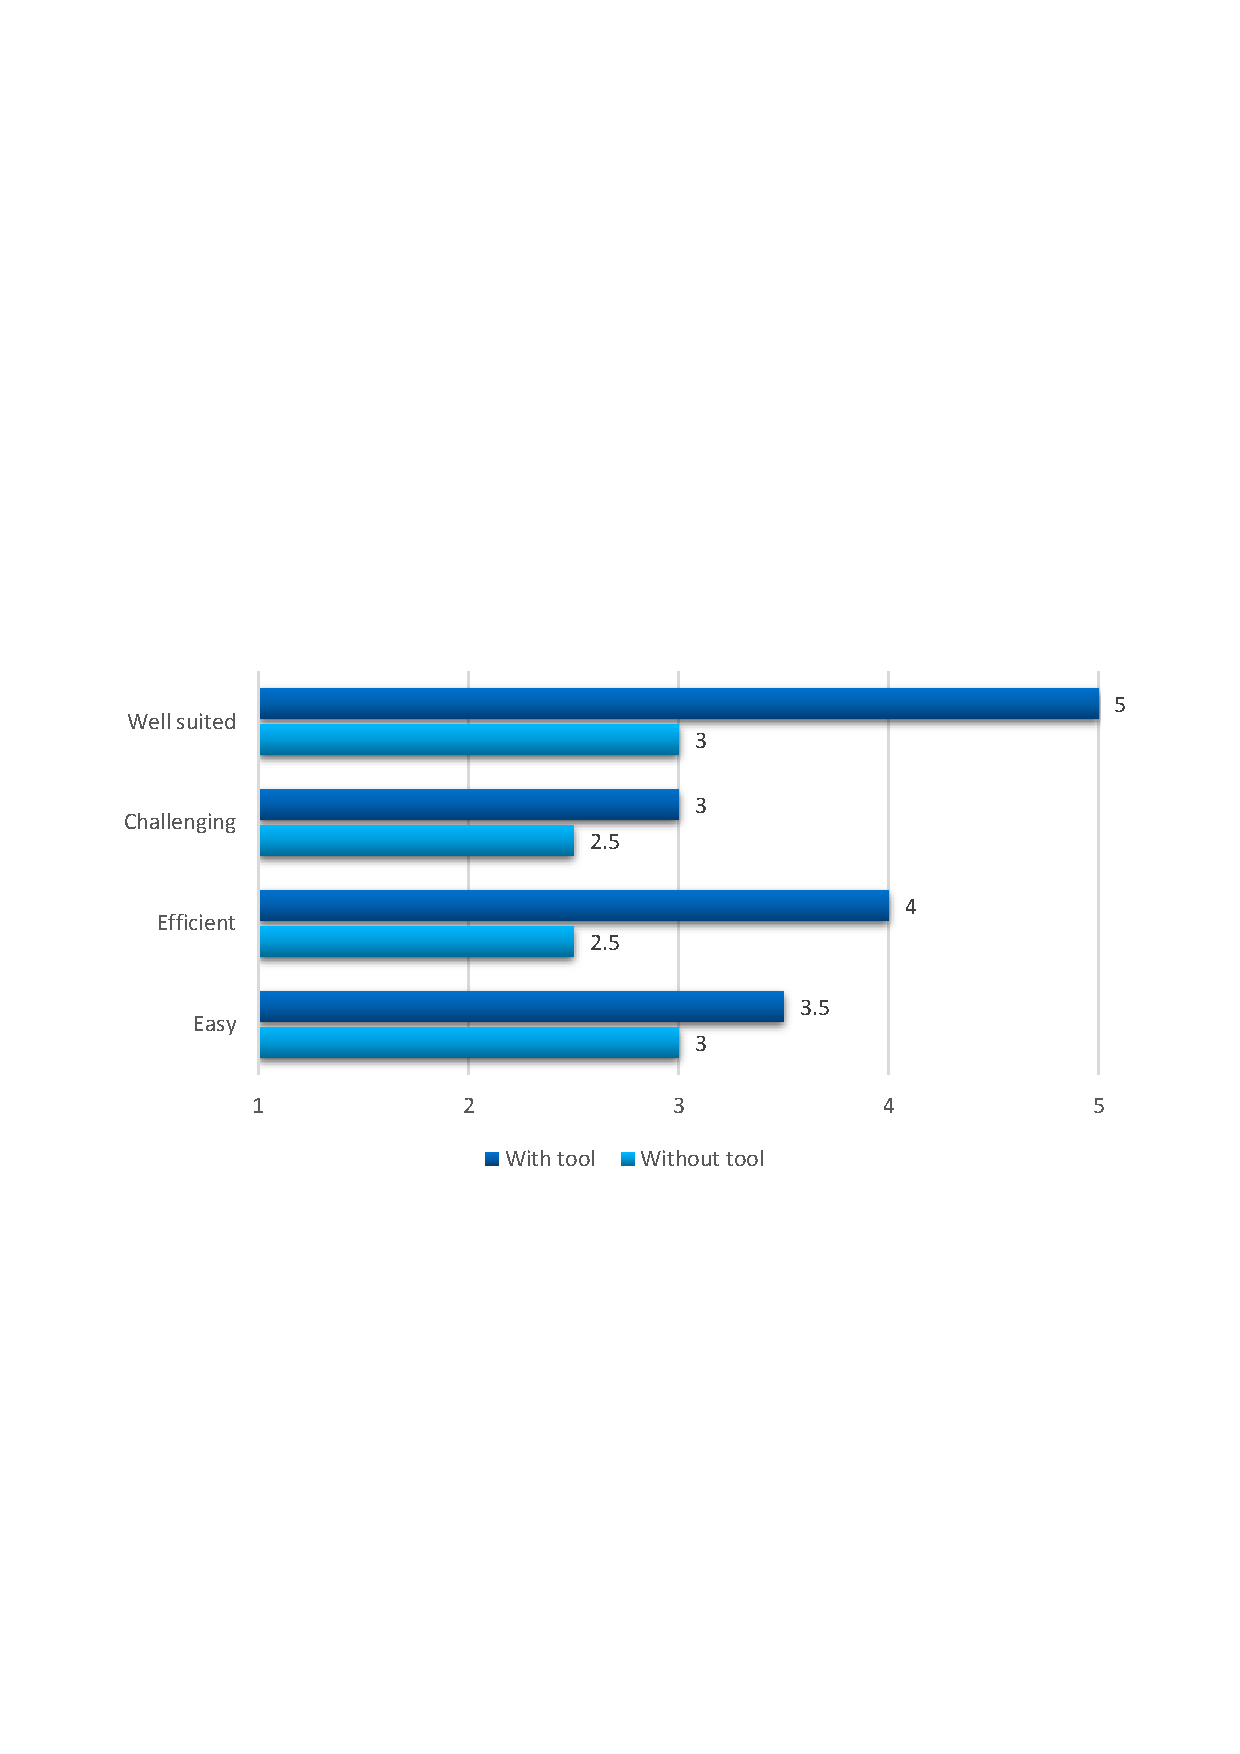
\includegraphics[width=0.8\textwidth]{images/charts/xdyt_bug_comparison.pdf}
	\caption{XDYouTube debugging task - Comparison}
	\label{fig:xdyt_bug_comparison}
\end{figure}

In Figure ~\ref{fig:xdyt_bug_features_used}; the use and ratings of the individual features can be seen. All of the participants used device emulation and connection features and rated them as useful. Function debugging was also used by almost all participants, probably because it was difficult to reproduce the bug and the participants wanted to see what was going on in the functions. About half the participants used the shared JavaScript console, mainly to see the error produced in the function that caused the bug. One participant connected the Nexus 7 to our tools and liked the feature, but no statement about the general usefulness of the feature can be made from just one participant. 

\begin{figure}[H]
  \centering
    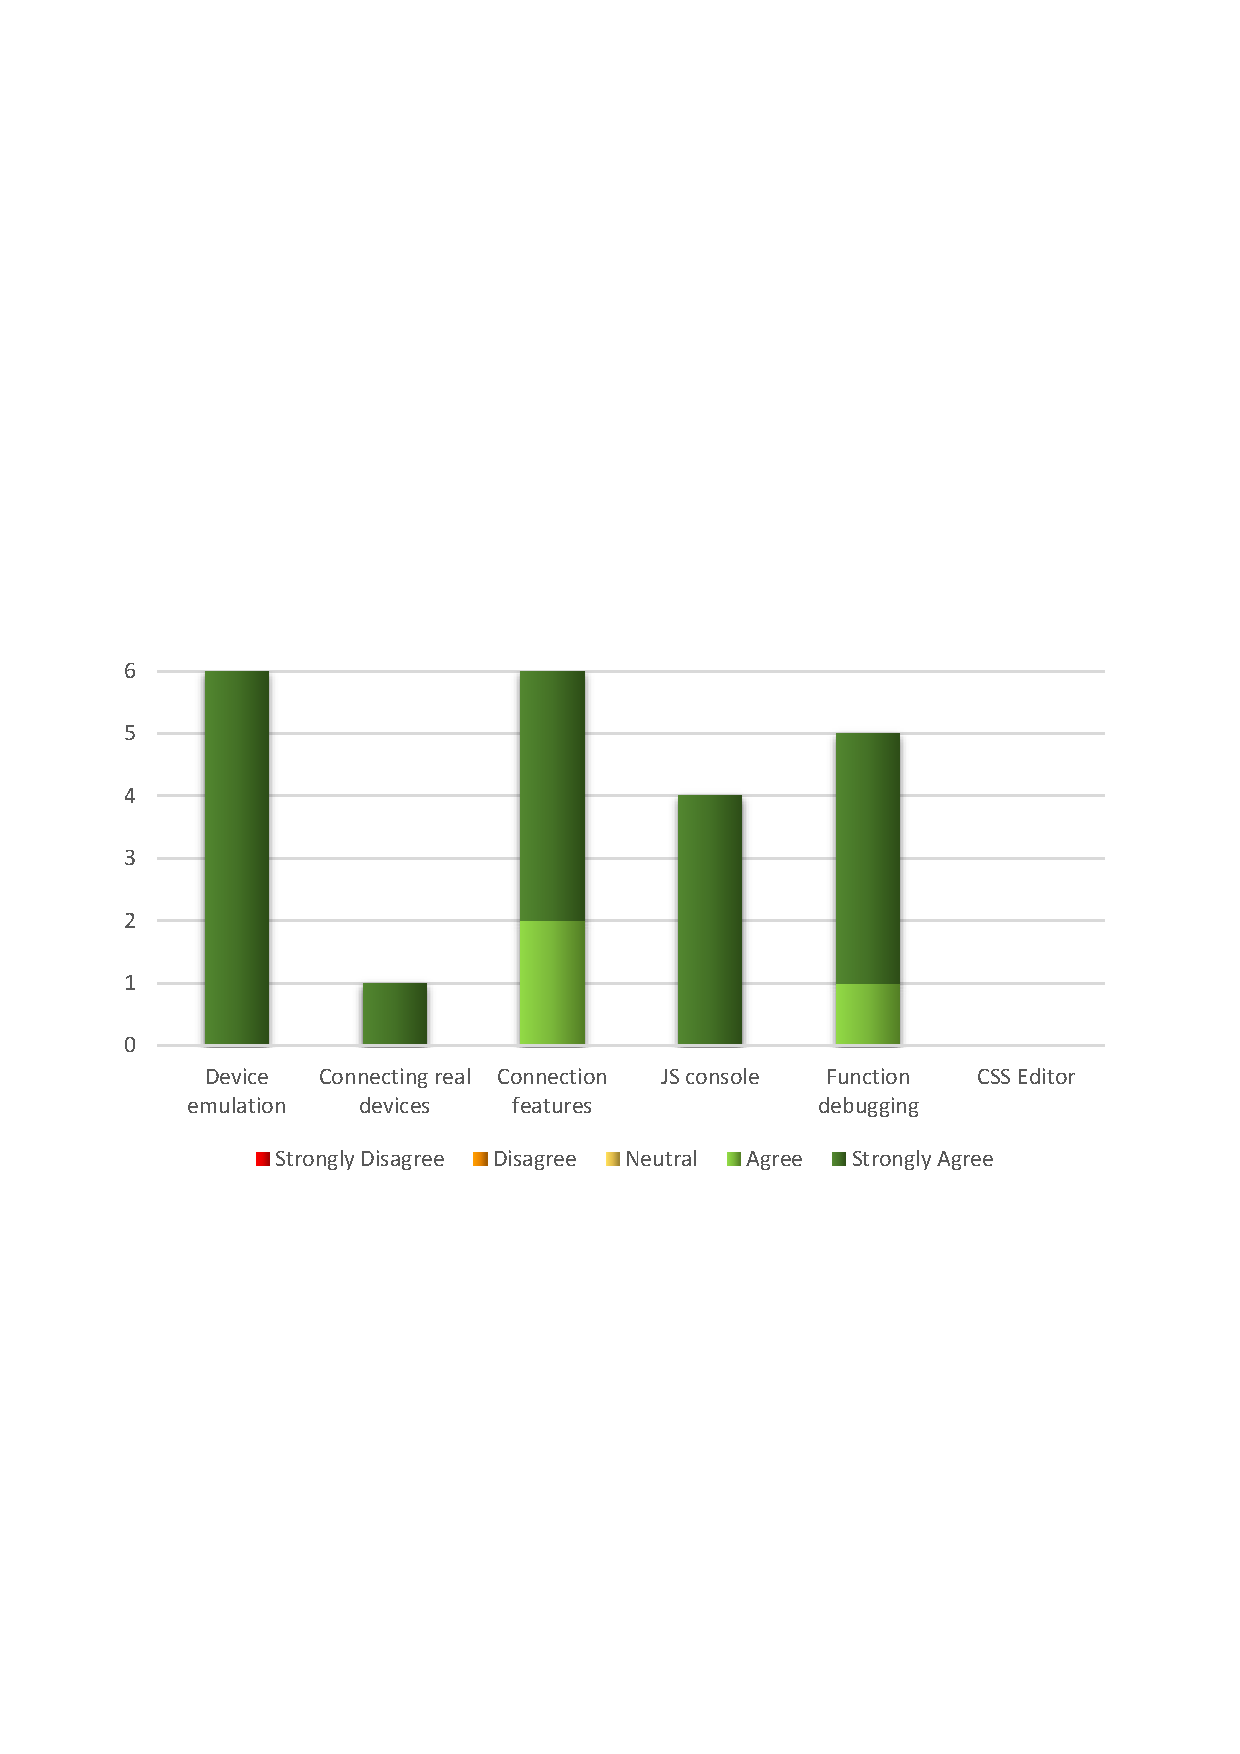
\includegraphics[width=0.8\textwidth]{images/charts/xdyt_bug_features_used.pdf}
	\caption{XDYouTube debugging task - Features used}
	\label{fig:xdyt_bug_features_used}
\end{figure}

\subsection{XDYouTube: Implementing a Feature}

Figure ~\ref{fig:xdyt_impl_comparison} shows the results for the implementation task in XDYouTube. In this task, all questions were clearly rated in favor of our tools. While the participant answered the questions in a rather neutral way when they did not have access to our tools, they clearly stated that the task was easy to complete and felt efficient to complete with our tools. This task differs from the others a bit, because all other tasks had questions where the difference in median was 0.5 or 0, whereas the difference is at least 1 in this task for every question. Especially in the questions concerning how challenging and how easy it was to complete a task, a big difference to the other three tasks can be seen. For the other three tasks, the difference between how challenging the task was was 0.5 for all tasks, and ranged from 0 to 1 regarding how easy it was to complete the task. In this task, the difference was 1.5 for both questions. Thus, this seems to be the only task where our tools made the task much easier to complete. One participant mentioned that they think that the XDYouTube tasks were better suited for the study because they emphasize the cross-device scenario more. If the other participants felt the same way about the task, this could be a possible explanation why they profited the most from our tools in this task.

\begin{figure}[H]
  \centering
    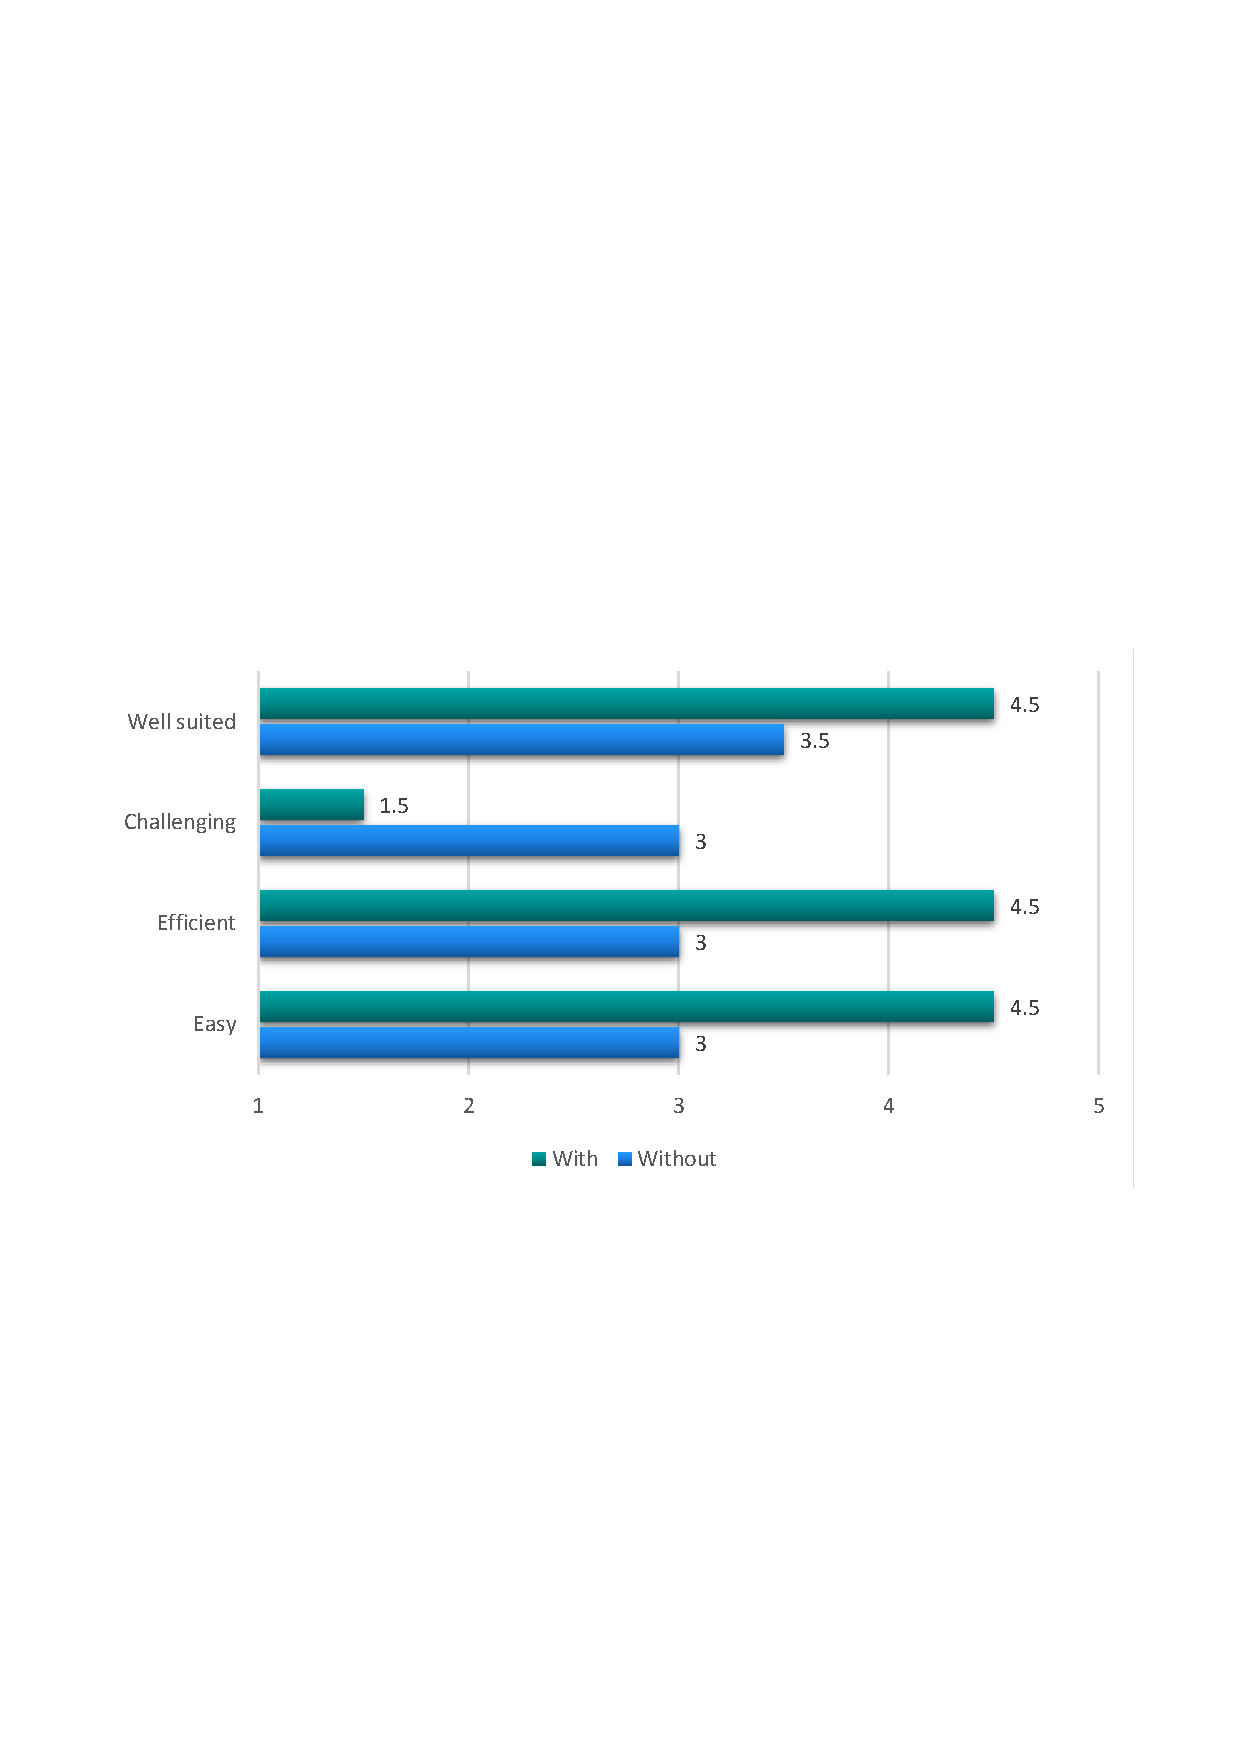
\includegraphics[width=0.8\textwidth]{images/charts/xdyt_impl_comparison.pdf}
	\caption{XDYouTube implementing task - Comparison}
	\label{fig:xdyt_impl_comparison}
\end{figure}

In Figure ~\ref{fig:xdyt_impl_features_used}; the use and ratings of the individual features can be seen. Once again, device emulation and the connection features were used by every participant. The shared JavaScript console and CSS editor were about equally popular and rated as very useful except for one participant that had a neutral opinion on the console. Function debugging was rarely used for this task. This is rather surprising because many participants had a bug where they had switched playing and pausing the video at the beginning and this could probably have been solved easily by debugging the function. However, most participants just got stuck at the bug and required some hints to fix it instead of debugging their functions.

\begin{figure}[H]
  \centering
    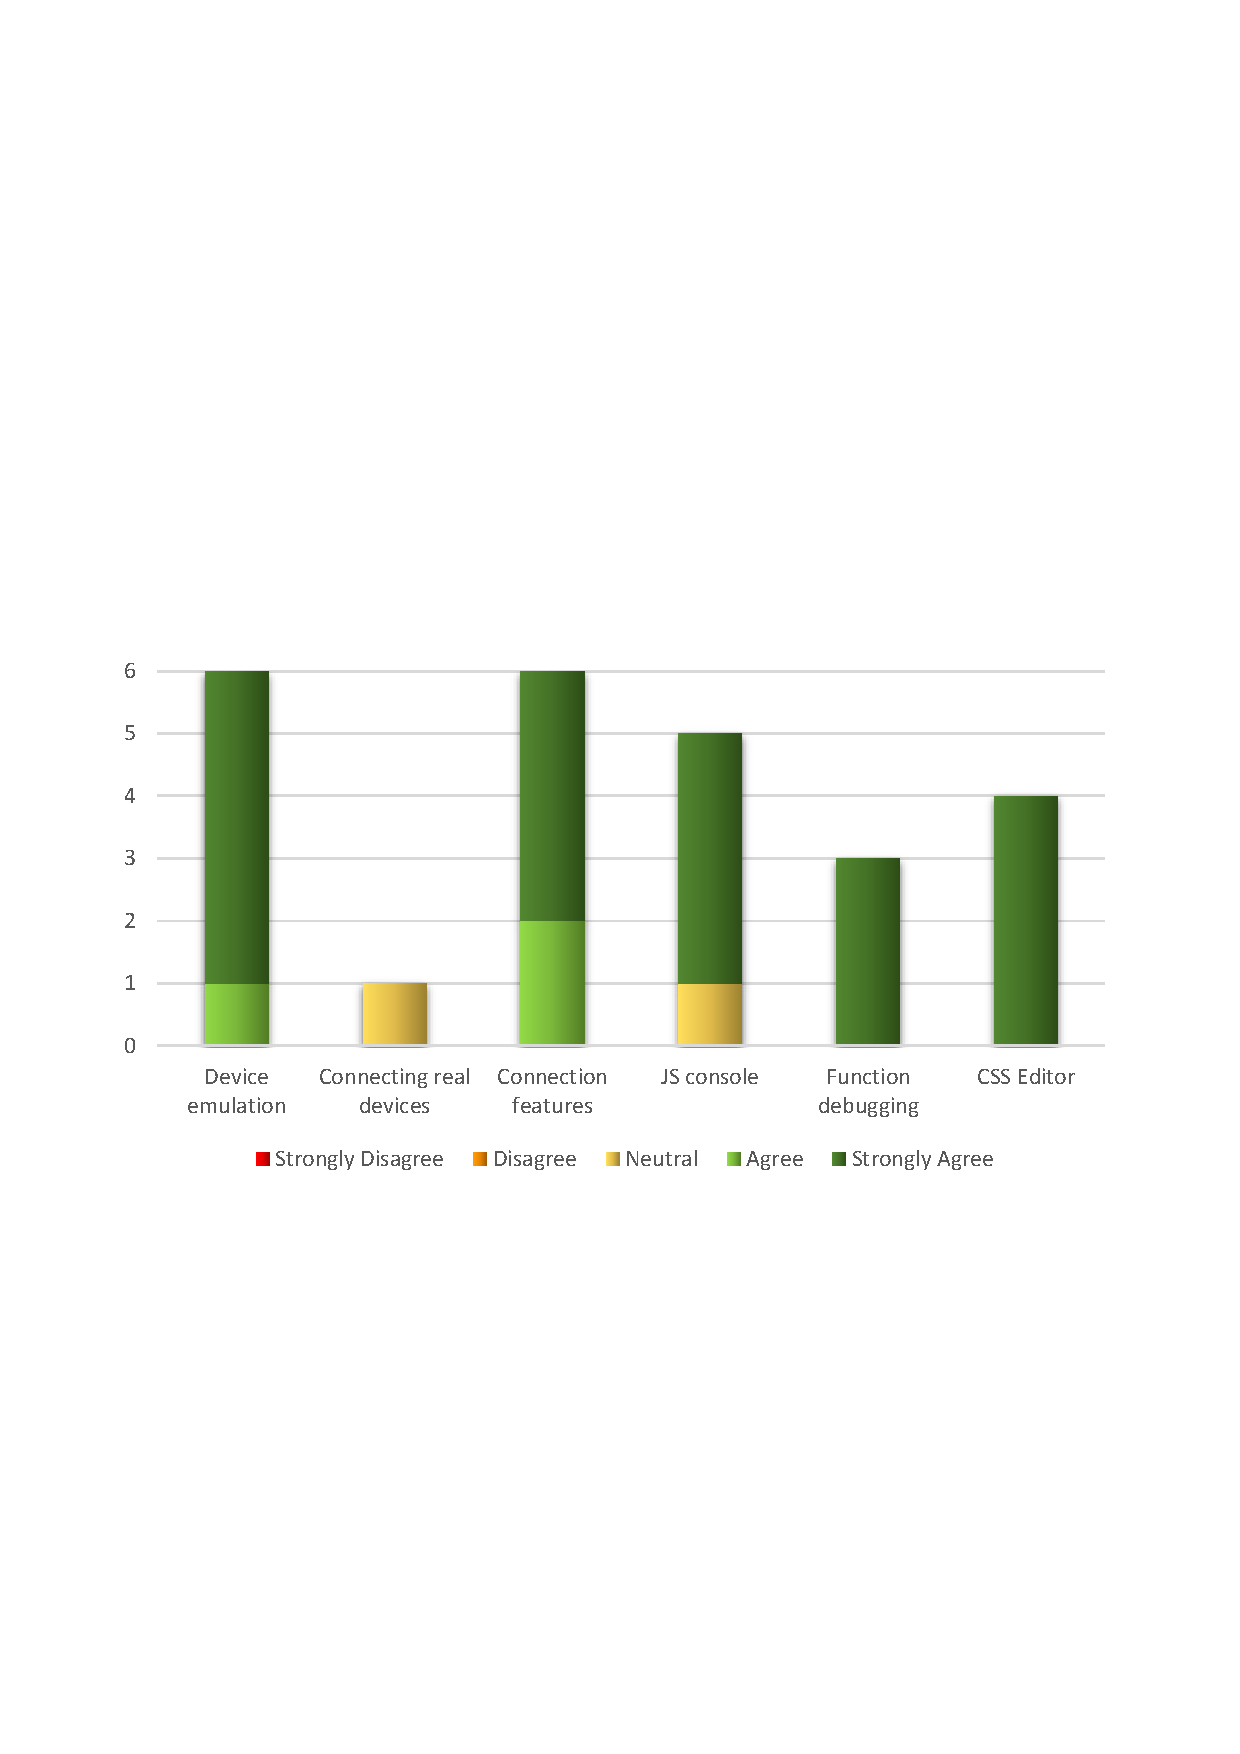
\includegraphics[width=0.8\textwidth]{images/charts/xdyt_impl_features_used.pdf}
	\caption{XDYouTube implementing task - Features used}
	\label{fig:xdyt_impl_features_used}
\end{figure}

\subsection{General}

In general, our tools were rated as very well suited for all tasks with a median value of 5 for each task except the XDYouTube implementation task where the median value is 4.5. In contrast, the usefulness of the usual browser tools was rated with median values between 3 and 4, this indicates that our tools are indeed better suited for implementing and debugging cross-device applications. The efficiency was also rated as significantly better for all tasks except the debugging task in XDCinema, where the difference was only 0.5. This indicates that our tools make the process of testing cross-device applications more efficient. The difference in easiness seems to depend partially on the type of task; in the tasks where the participants had to implement a feature, completing the task with our tools was clearly considered easier, whereas the difference was smaller for the tasks where the participants had to fix a bug. Surprisingly, the results for the question about how challenging it was to complete the task do not necessarily relate to the results of the question about easiness. For all tasks except the XDYouTube implementation task, the differences are very minor, thus our tools do not seem to have much influence on how challenging a task is perceived.

Without our tools, it looks like participant considered the XDYouTube tasks as more difficult than the XDCinema tasks. This generally corresponds to what participants said during the study. While most of them did not make any comments about the difficulty of the task, those who did said that the XDYouTube tasks were more difficult. However, when using our tools, the picture looks a bit different. With access to our tools, it seems that the debugging tasks are considered harder than the implementation tasks. In principle, this is the opposite of what we wanted to achieve, as the debugging tasks were designed as "introduction" tasks. However, the completion times show that the participants were not actually faster when completing the implementation tasks than when completing the debugging tasks, therefore the different results in the questionnaires can be considered as okay. Surprisingly, the difference in median values for the question where we asked how well suited the tools were for the tasks is larger in the debugging tasks than in the implementation tasks. The difference is 1 for both implementation tasks and 1.5 and 2 for the debugging tasks. Thus, the participants that had access to our tools considered the debugging tasks as more difficult than the implementation tasks, but still felt that our tools were much better suited than the usual browser tools. So far, those results make sense: If the task is more difficult, the user can profit more from our tools. However, what remains to be explained is why the participants that did not have access to our tools found the XDYouTube tasks more difficult than the XDCinema task. The explanation lies in the XDYouTube implementation task: As mentioned before, participants seem to profit the most of our tools in this tasks. Consequently, our tools make the task so much easier that it is no longer considered one of the more difficult tasks by the participants that have access to our tools. However, the XDCinema bug was not really perceived as easier to complete with our tools, thus it is one of the more challenging tasks for the participants that had access to our tools, but not for the participants that did not have access to our tools.

\section{Discussion}

Figure ~\ref{fig:implementing_easier} shows that about three quarters of all participants considered implementing a feature easier with our tools. Only one participant found it easier to implement a feature without our tools. However, in principle, this option is redundant as the participants still have access to the browser tools even when they have access to our tools. Thus the relevant conclusion is that about one quarter of the participants did not see any gain in easiness from using our tools. The same applies to the question about whether implementing a feature feels more efficient with our tools (see Figure ~\ref{fig:implementing_efficient}); this figure shows exactly the same results as the figure about easiness. However, all except one participant preferred implementing a feature with our tools (see Figure ~\ref{fig:prefer_implementing}). Thus, it seems that participants like to have access to our tools even if they cannot directly relate them to a decrease in difficulty or to an increase in efficiency.
\begin{figure}[H]
  \centering
    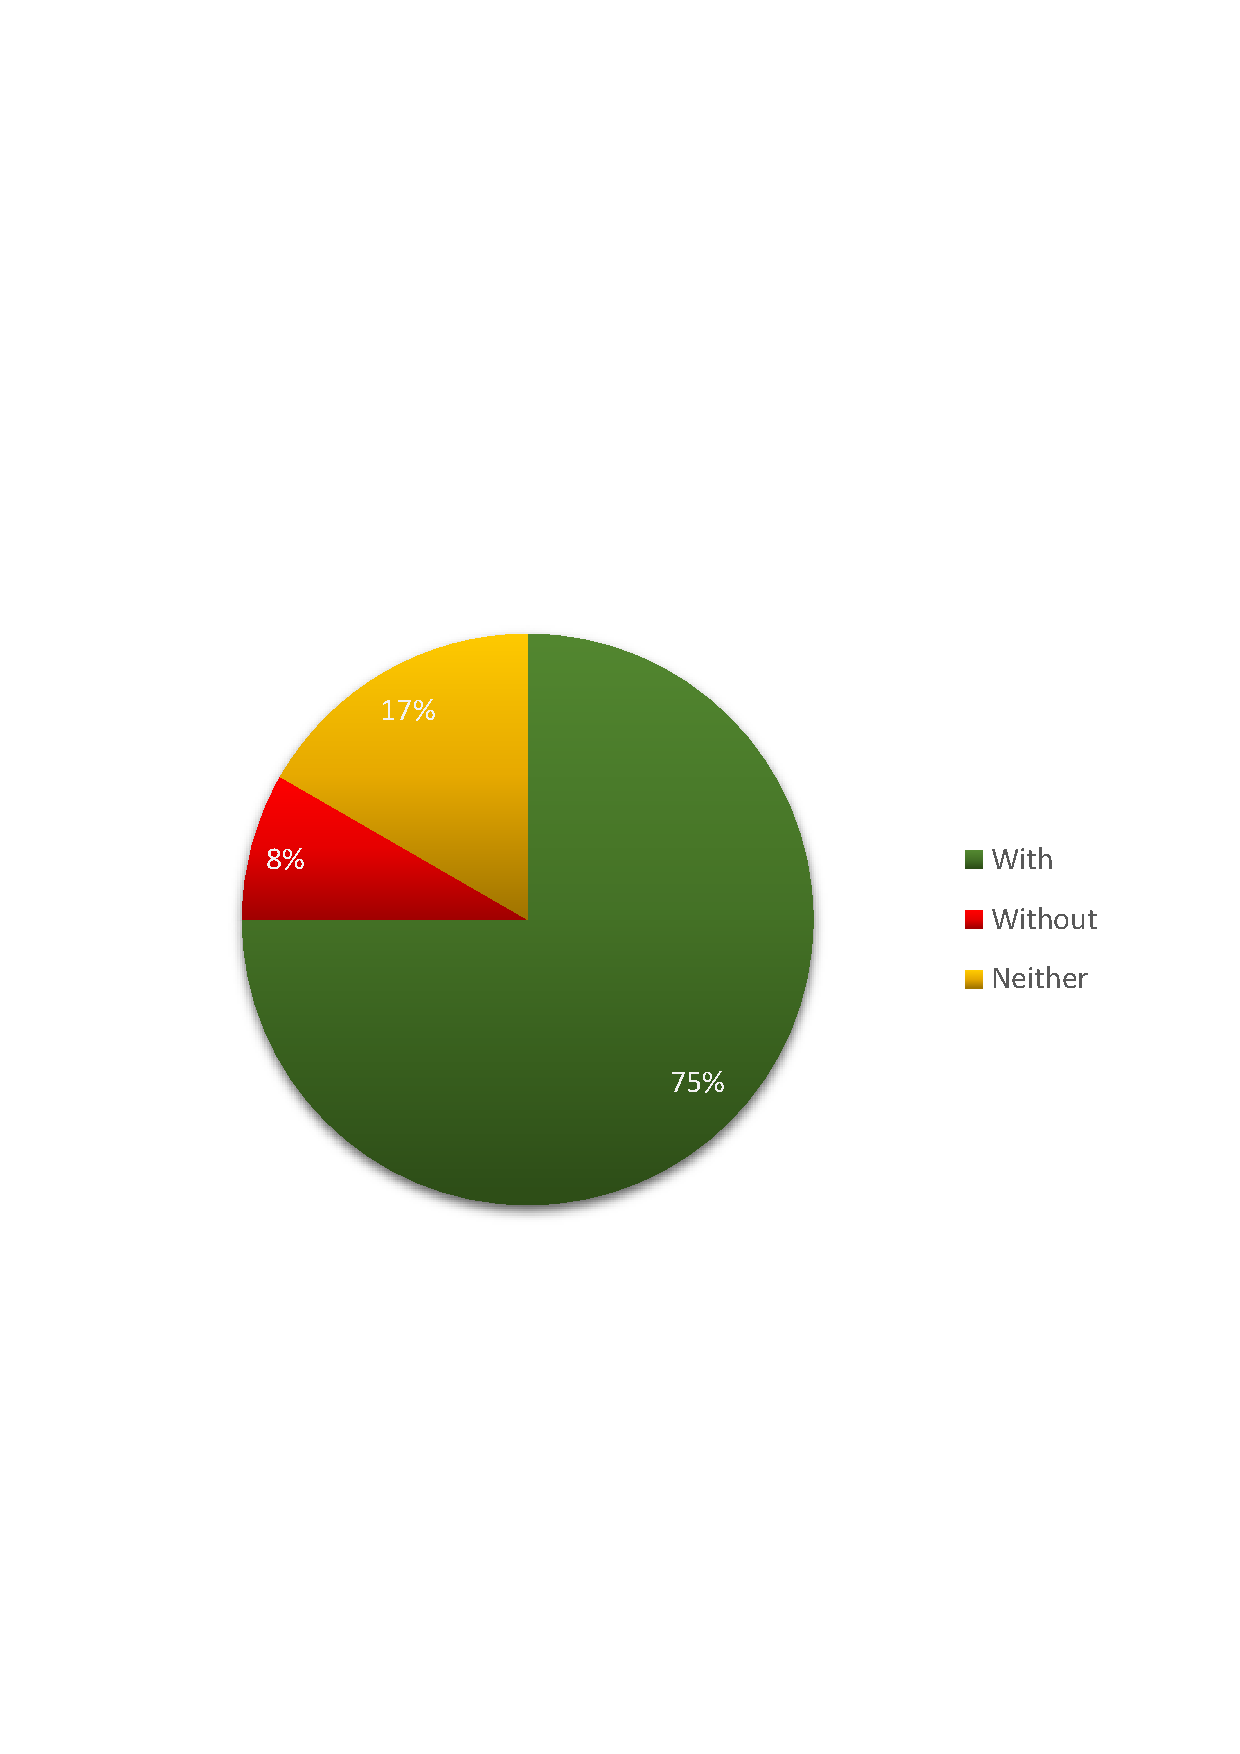
\includegraphics[width=0.6\textwidth]{images/charts/implementing_easier.pdf}
	\caption{Easiness of implementing a feature}
	\label{fig:implementing_easier}
\end{figure}

\begin{figure}[H]
  \centering
    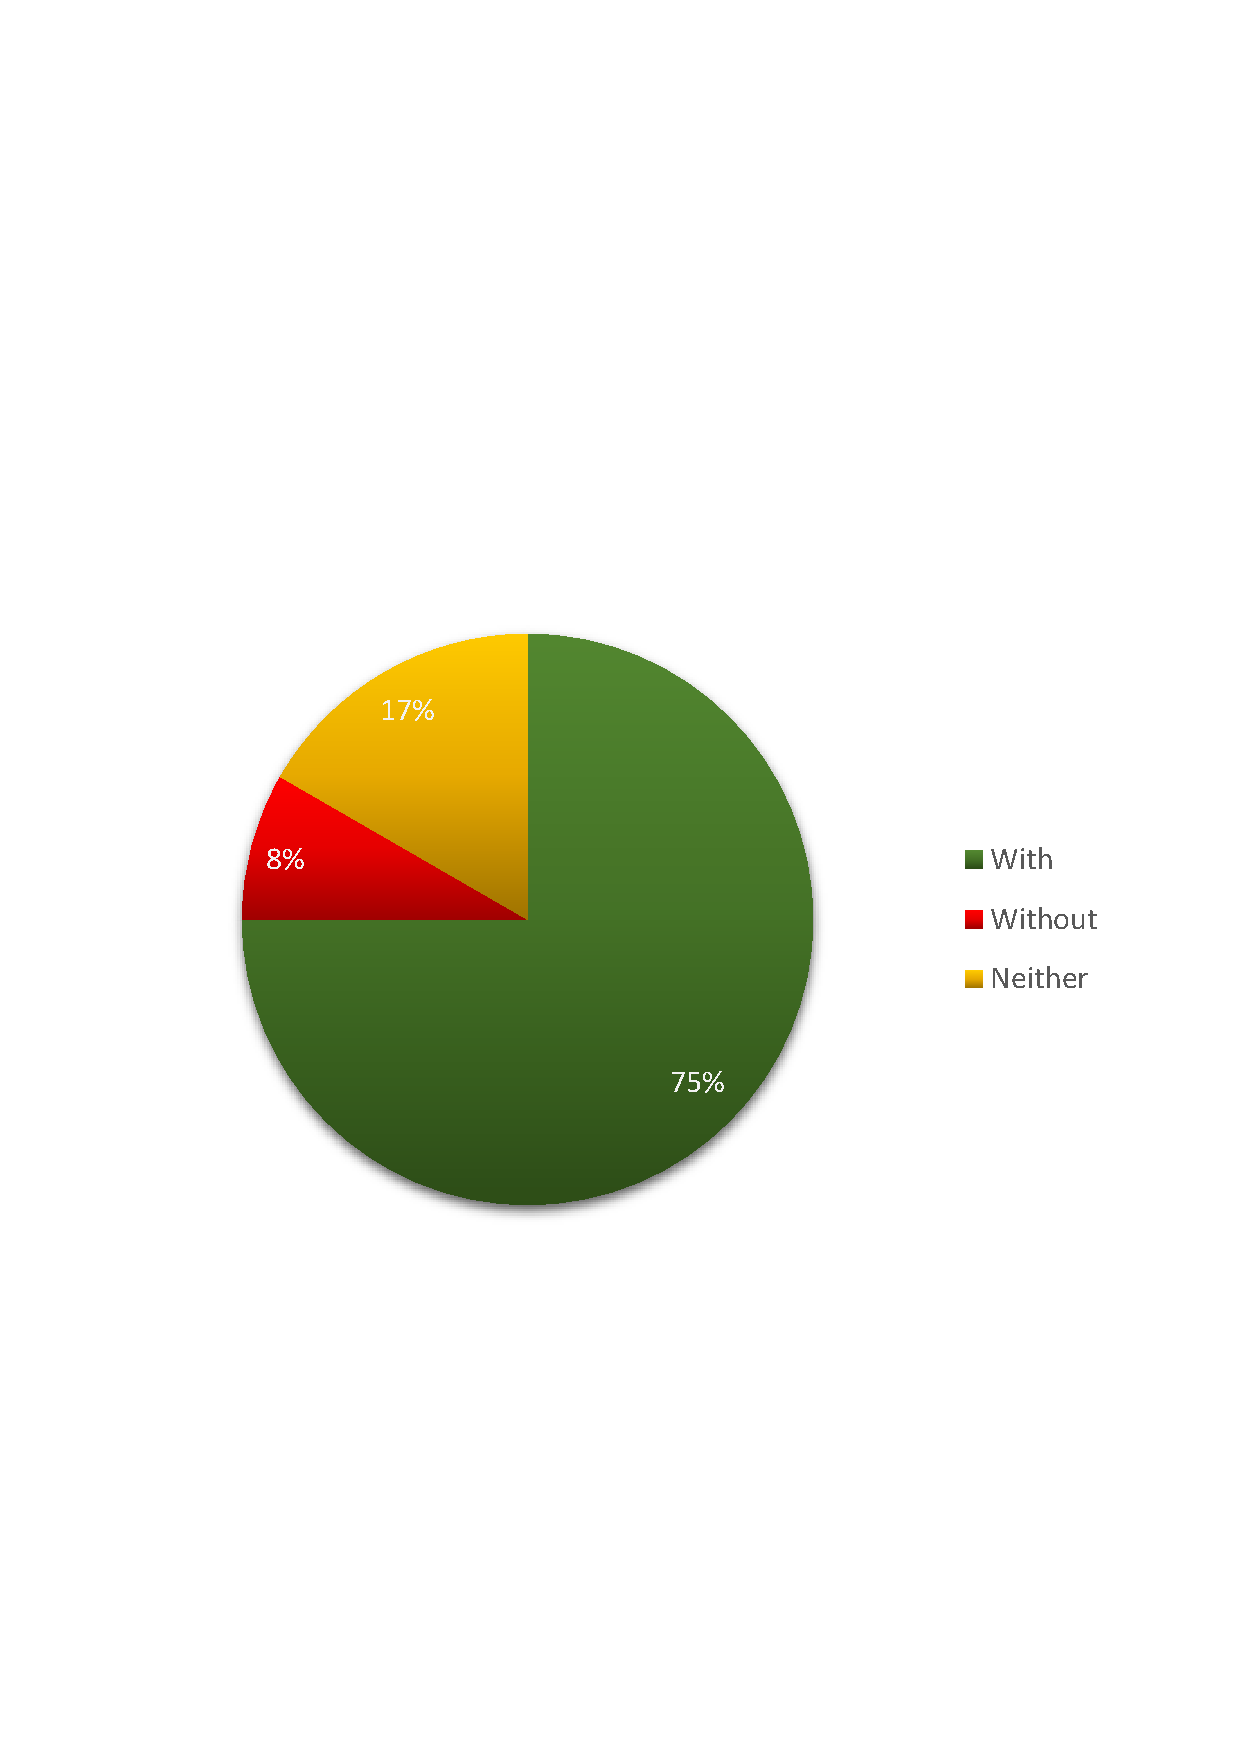
\includegraphics[width=0.6\textwidth]{images/charts/implementing_efficient.pdf}
	\caption{Efficiency of implementing a feature}
	\label{fig:implementing_efficient}
\end{figure}

\begin{figure}[H]
  \centering
    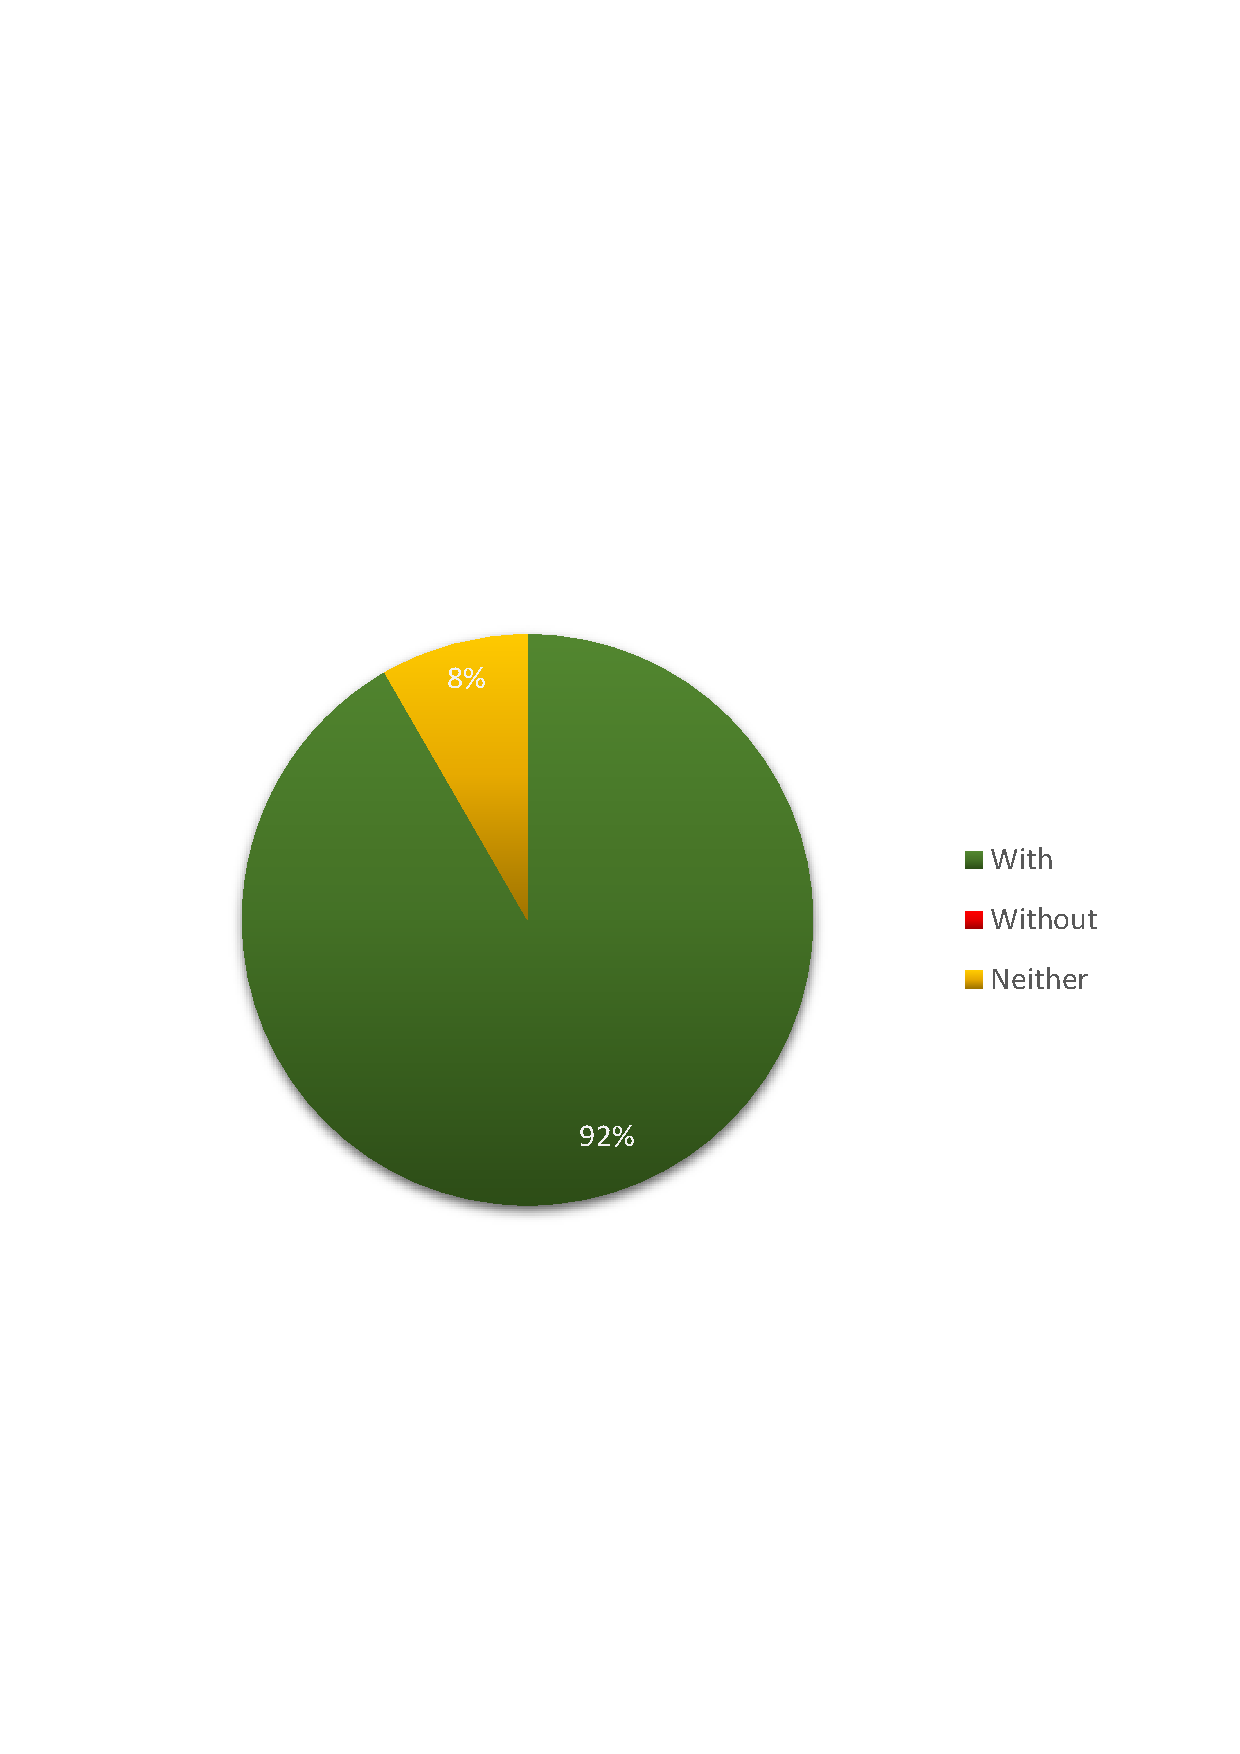
\includegraphics[width=0.6\textwidth]{images/charts/prefer_implementing.pdf}
	\caption{Preference for implementing a feature}
	\label{fig:prefer_implementing}
\end{figure}

Figure ~\ref{fig:debugging_easier} shows that most participants found it easier to debug a cross-device application with our tools. The results get even more obvious if we look at Figure ~\ref{fig:debugging_efficient} and Figure ~\ref{prefer_debugging}. Those two figures show that all participants felt more efficient when debugging with our tools and also preferred debugging with our tools.

\begin{figure}[H]
  \centering
    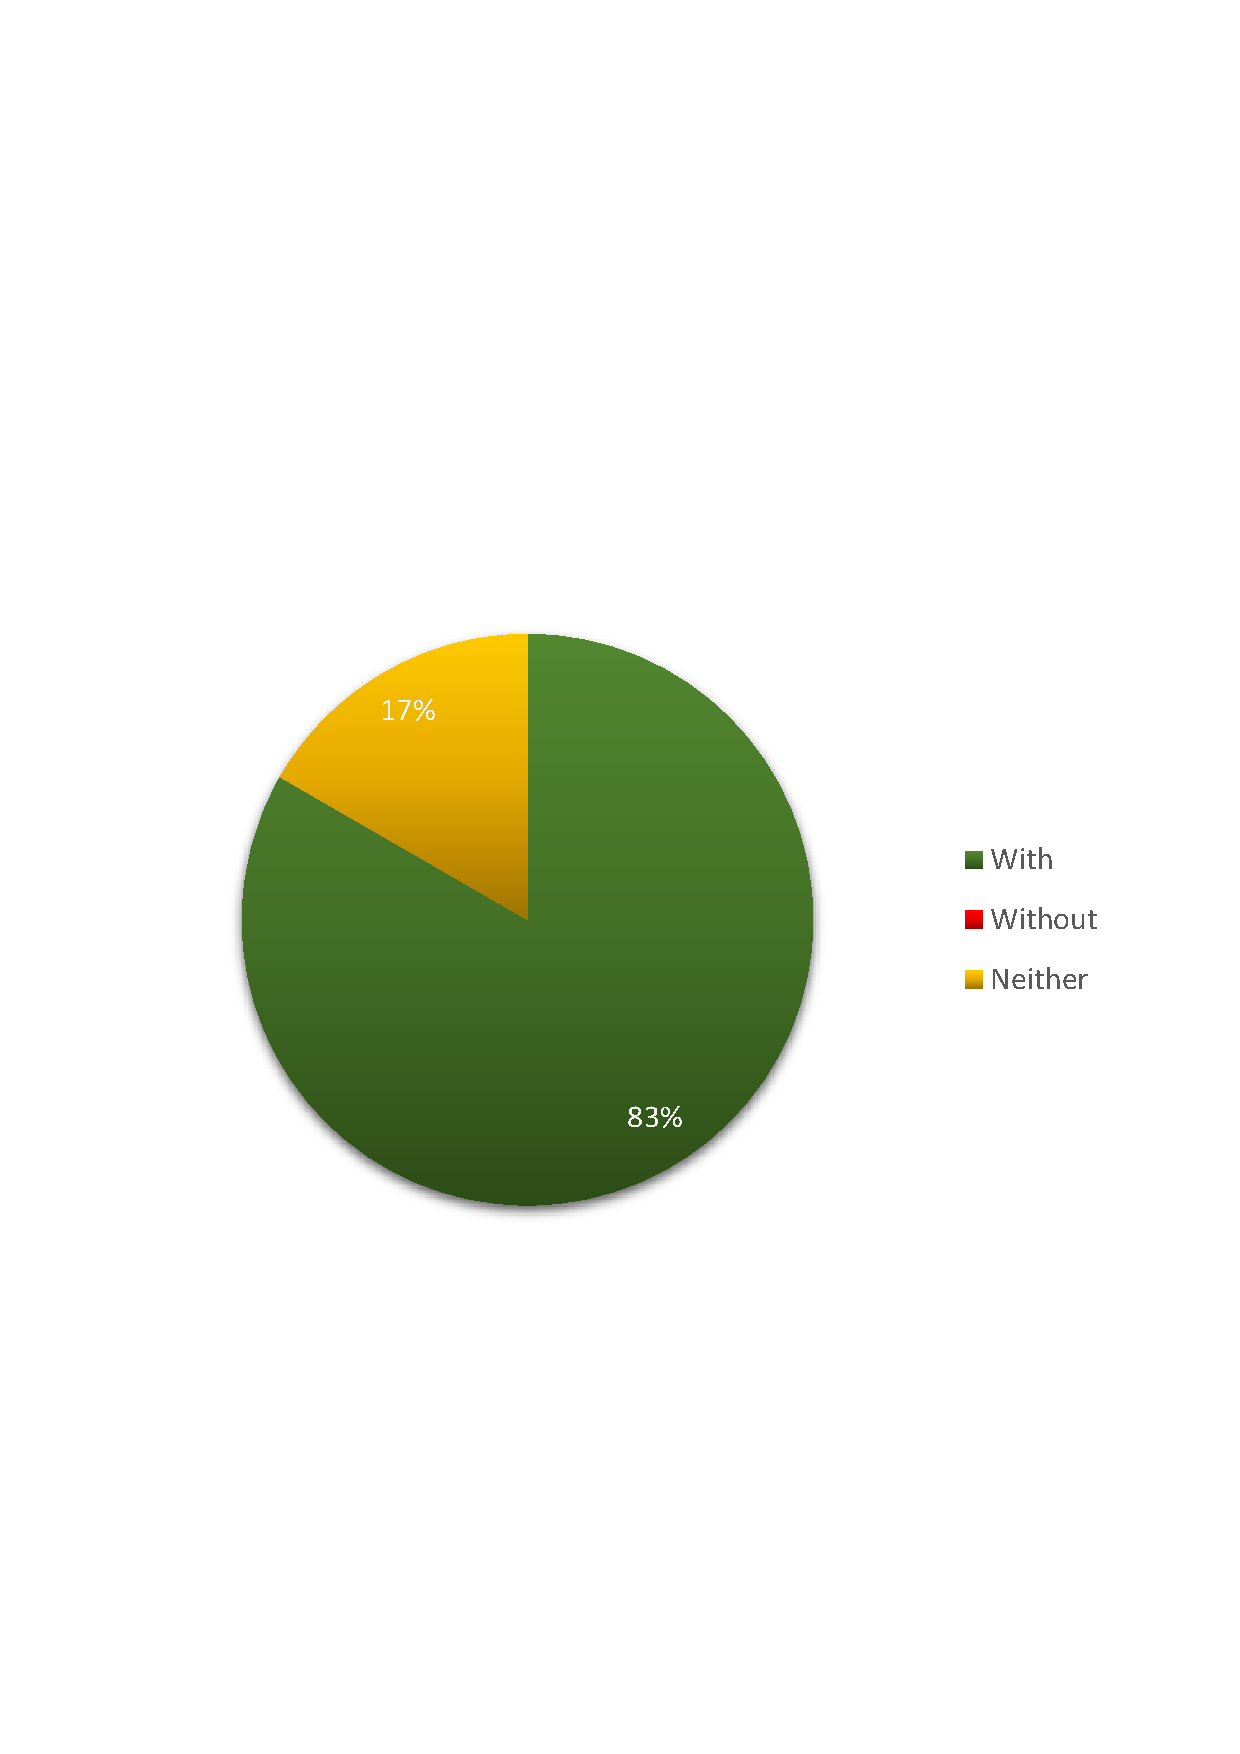
\includegraphics[width=0.6\textwidth]{images/charts/debugging_easier.pdf}
	\caption{Easiness of debugging}
	\label{fig:debugging_easier}
\end{figure}

\begin{figure}[H]
  \centering
    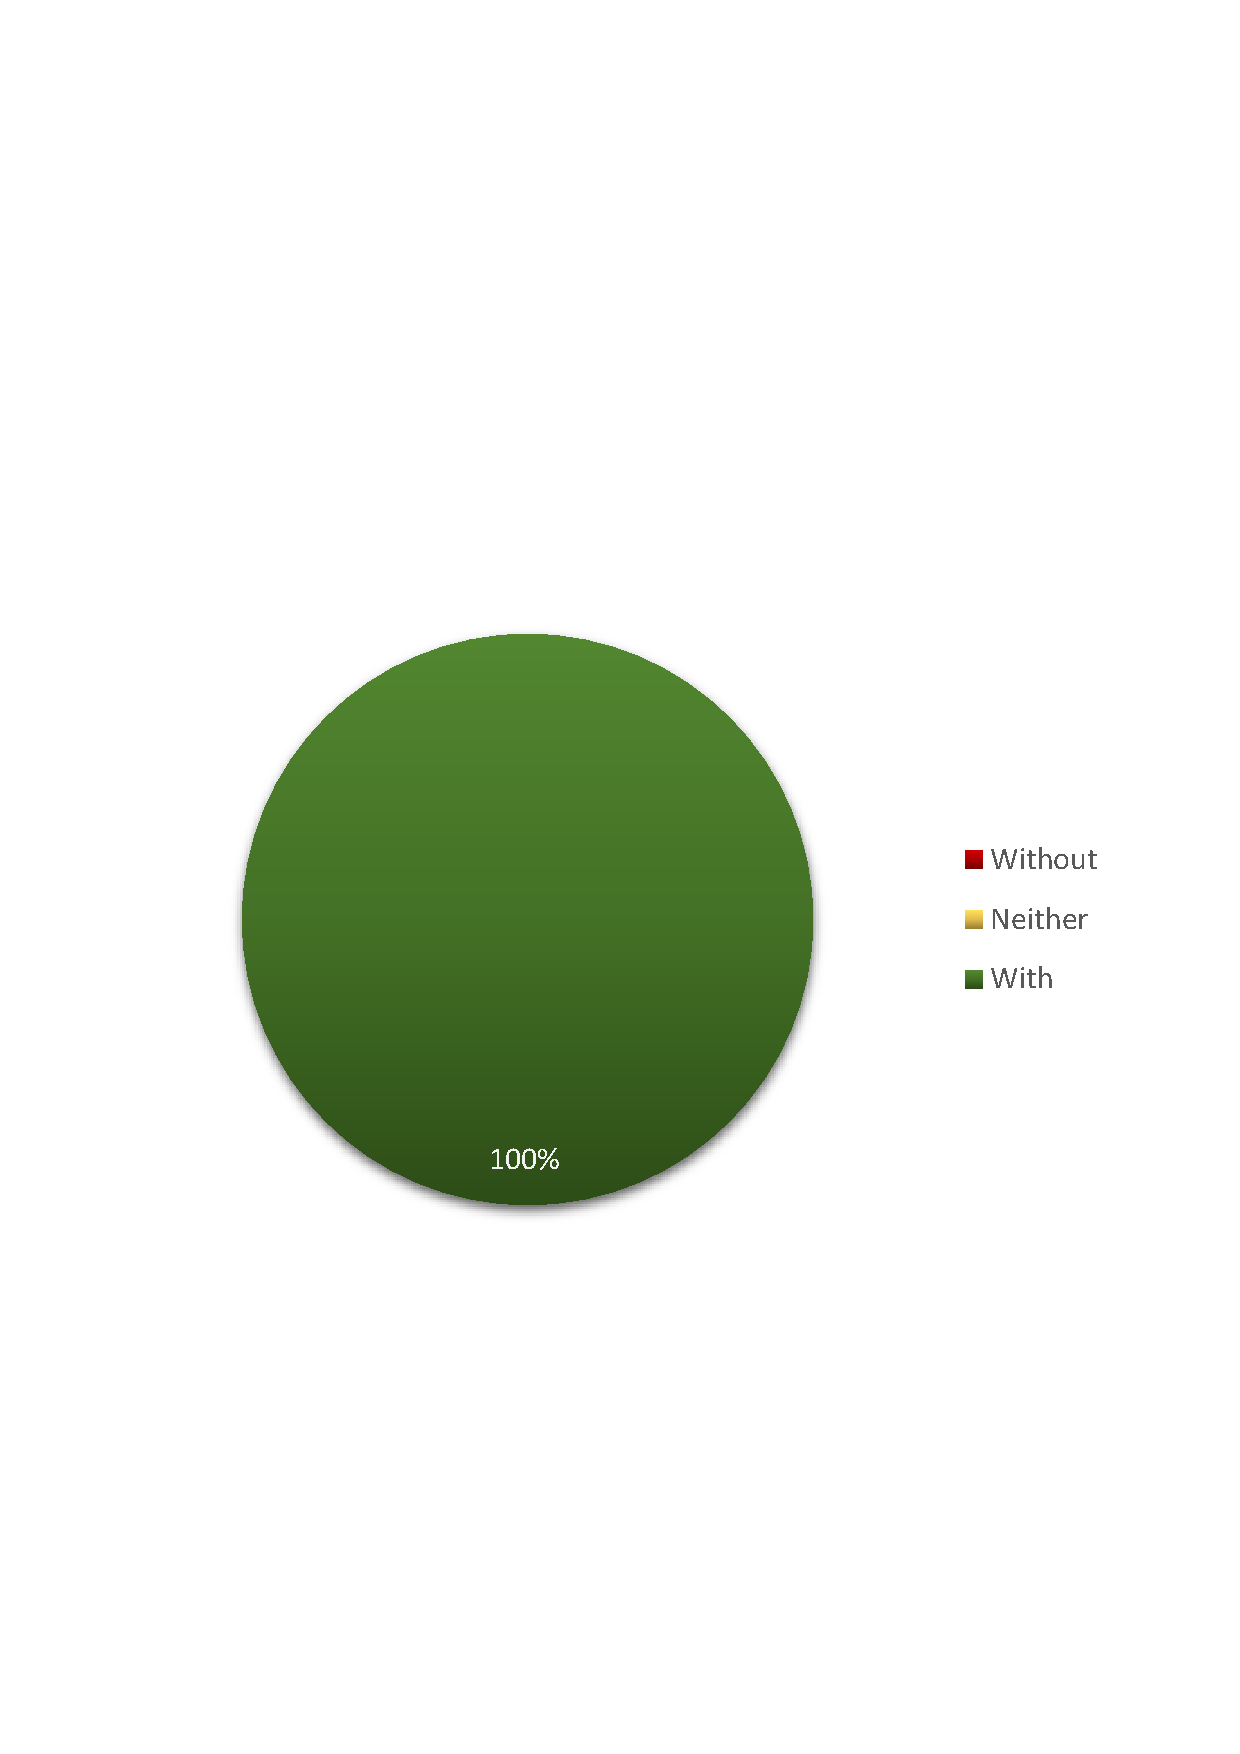
\includegraphics[width=0.6\textwidth]{images/charts/debugging_efficient.pdf}
	\caption{Efficiency of debugging}
	\label{fig:debugging_efficient}
\end{figure}

\begin{figure}[H]
  \centering
    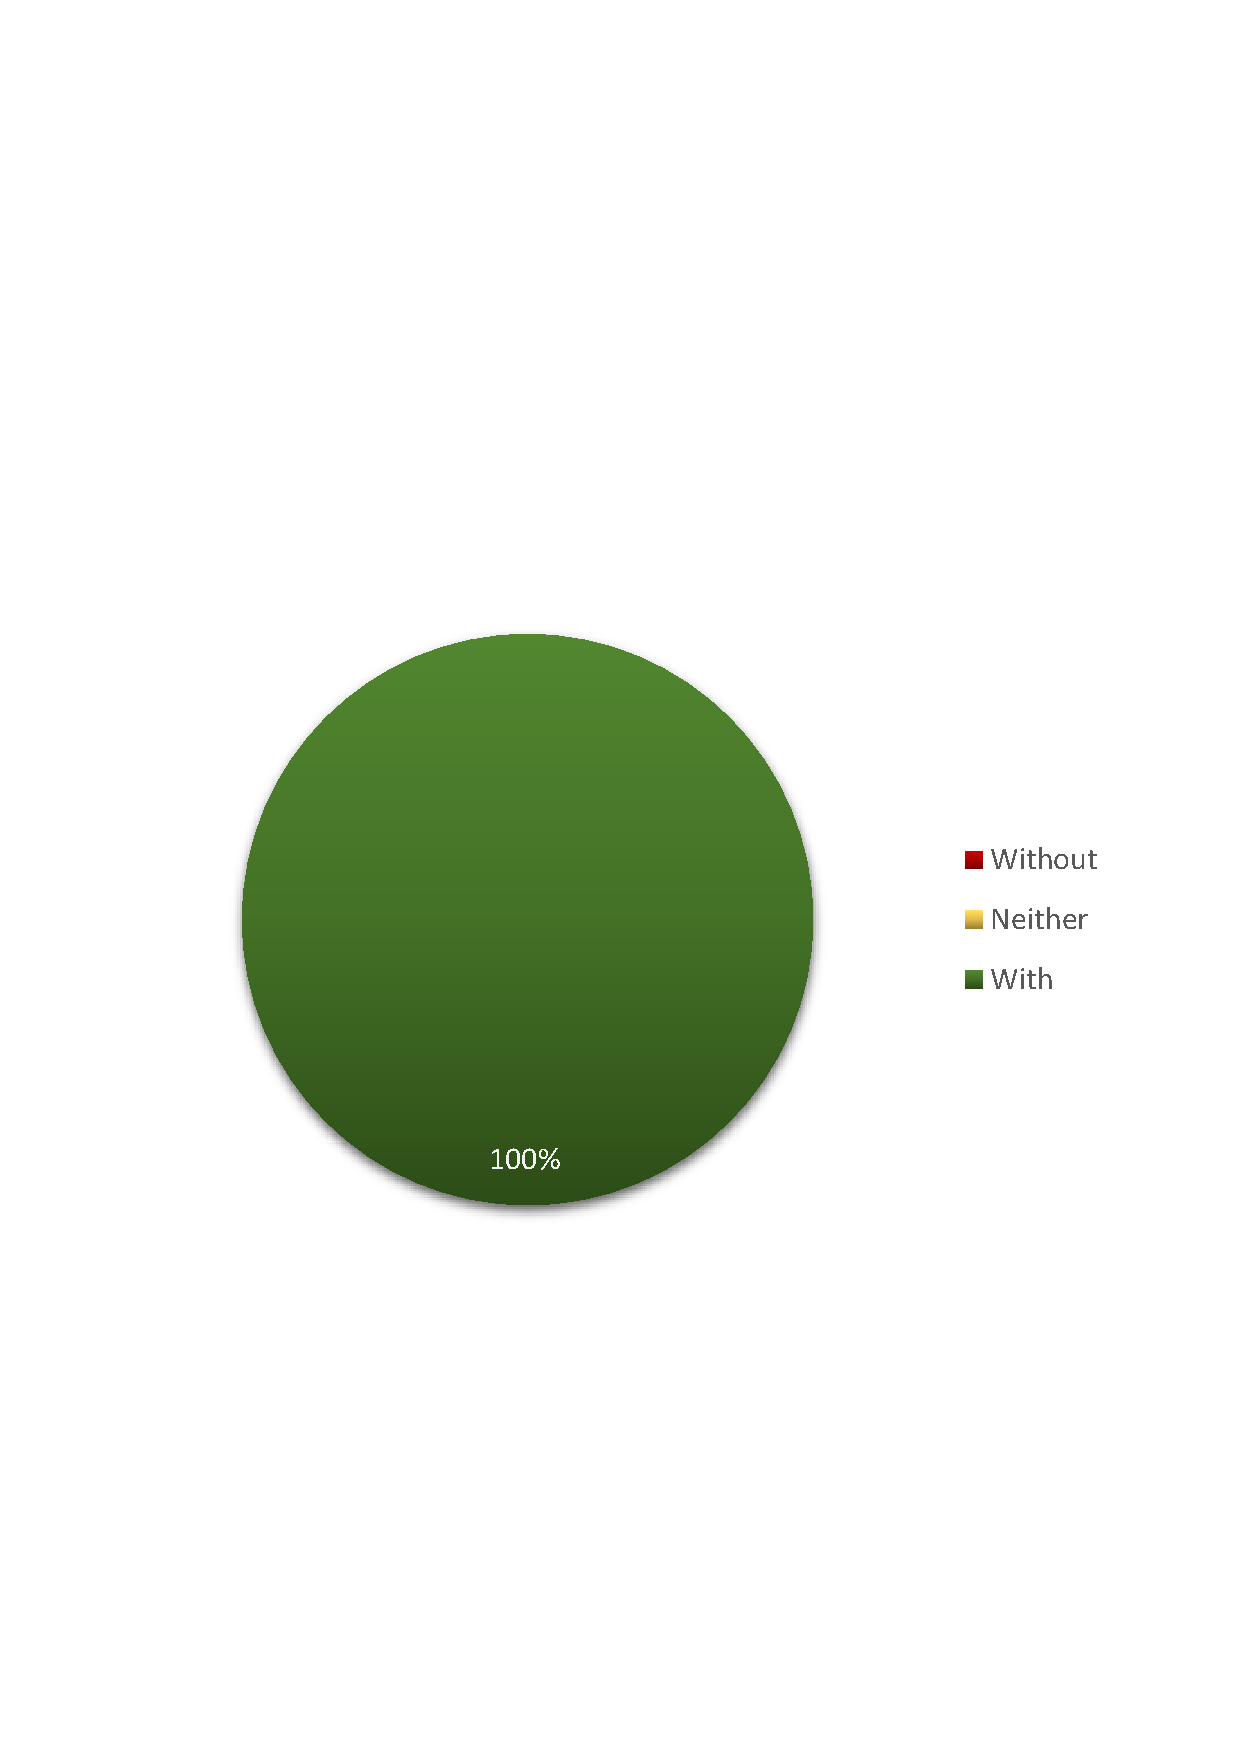
\includegraphics[width=0.6\textwidth]{images/charts/prefer_debugging.pdf}
	\caption{Preference for debugging}
	\label{fig:prefer_debugging}
\end{figure}


We also asked the participants if they would use our tools for debugging and implementing cross-device applications and if they think that our tools would be useful for cross-device application testing. The results can be seen in figure ~\ref{fig:usefulness_tool}. Almost all participants think that our tools would be very useful for implementing as well as debugging cross-device applications and the remaining few also think that they would be useful. All participants would use our tools for implementing cross-device applications and all except one participant would use them for debugging cross-device applications. A few more participants stated that they strongly agree with the statement that they would use our tools for debugging than for implementing. This is consistent with our previous results, where all participants preferred debugging with our tools but about one quarter did not prefer implementing with our tools.

\begin{figure}[H]
  \centering
    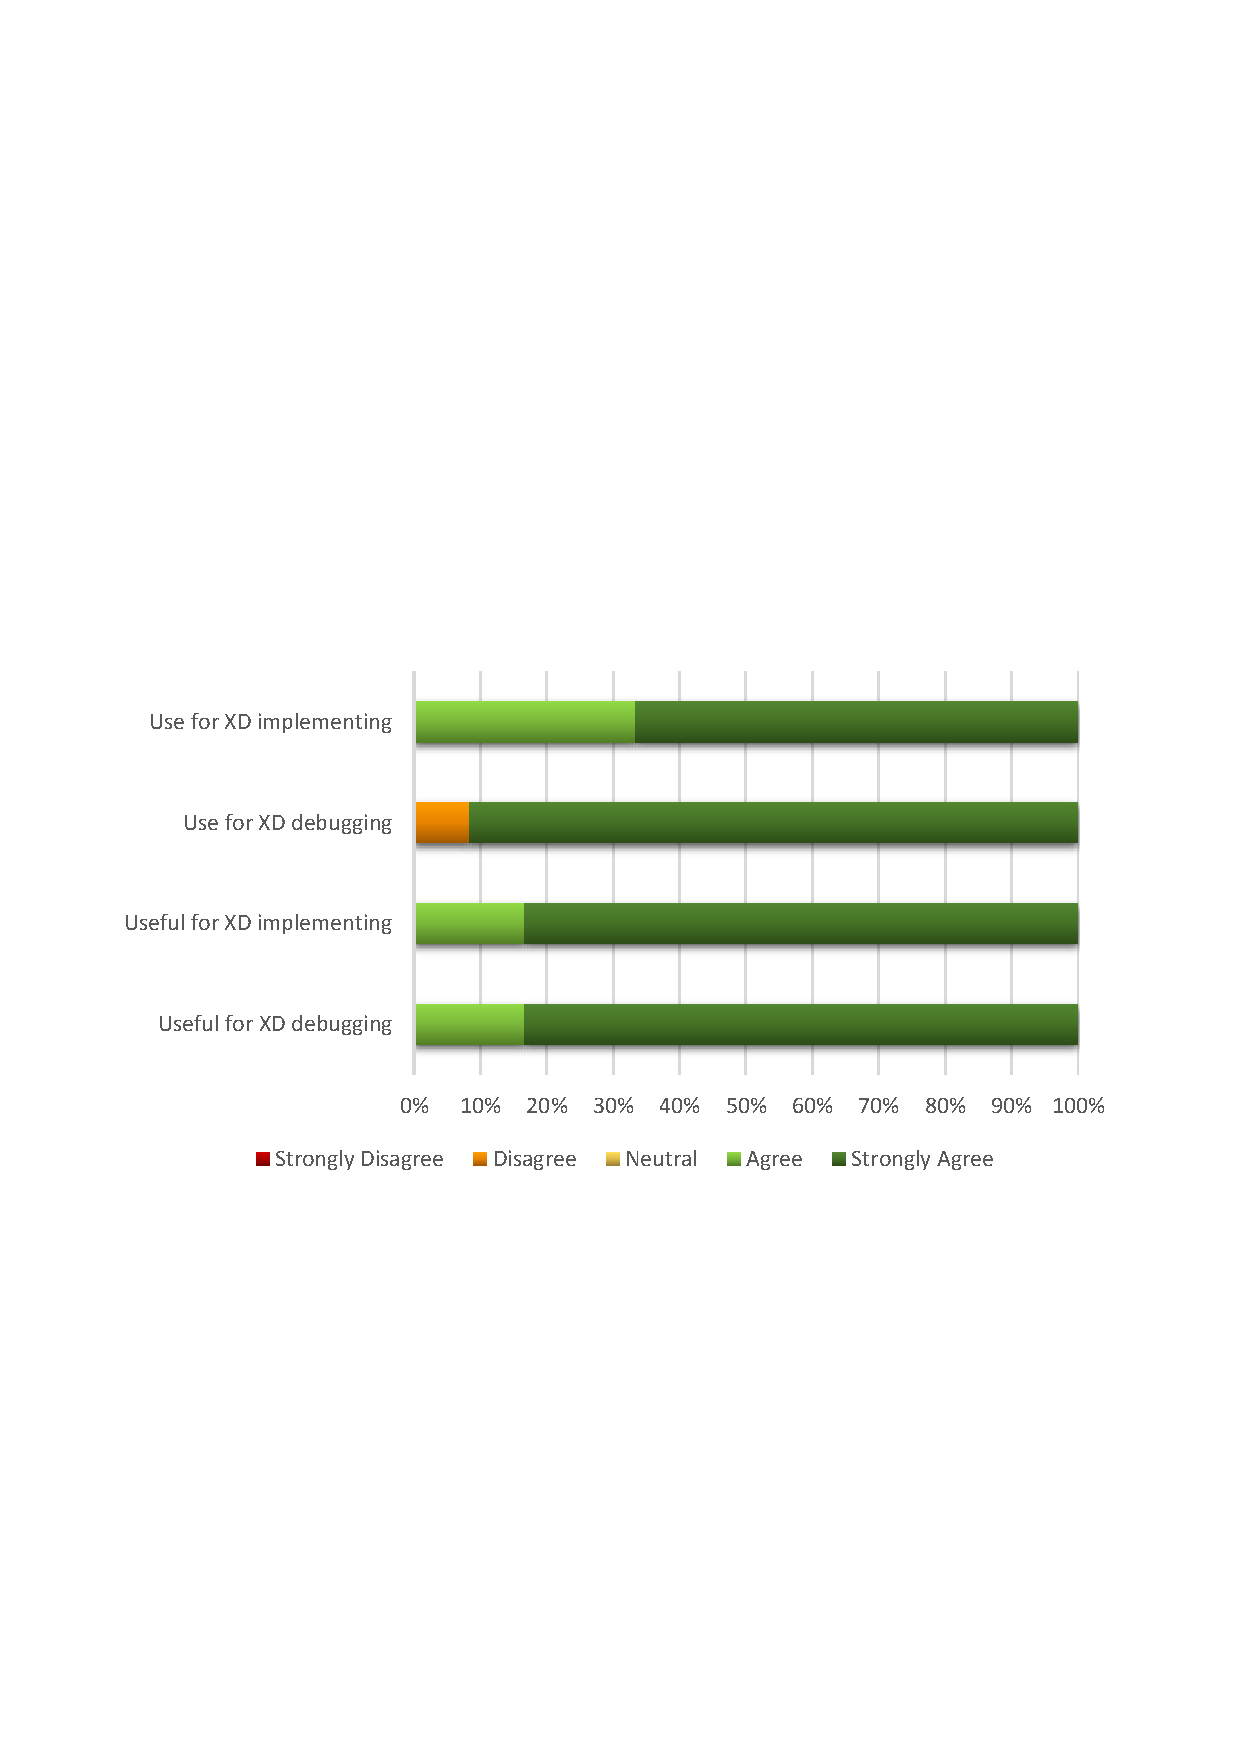
\includegraphics[width=0.8\textwidth]{images/charts/usefulness_tool.pdf}
	\caption{Usefulness of our tools}
	\label{fig:usefulness_tool}
\end{figure}

Finally, you can see the results for the general questions about our tools in Figure ~\ref{fig:tool_general}. The figure shows that our tools were perceived as easy to learn despite the many different features and the participants also felt rather confident using our tools. However, some participants rated the question about confidence in a neutral way and most other participants felt only somewhat confident, but not very confident. This indicates that even though our tools are considered easy to learn, it may still take participants some time to get used to them. Our tools are not considered as unnecessarily complex by almost all participants. The results of those three questions indicate that the interface of our tools is generally well-structured and it would be easy for developers to get used to our tools.

\begin{figure}[H]
  \centering
    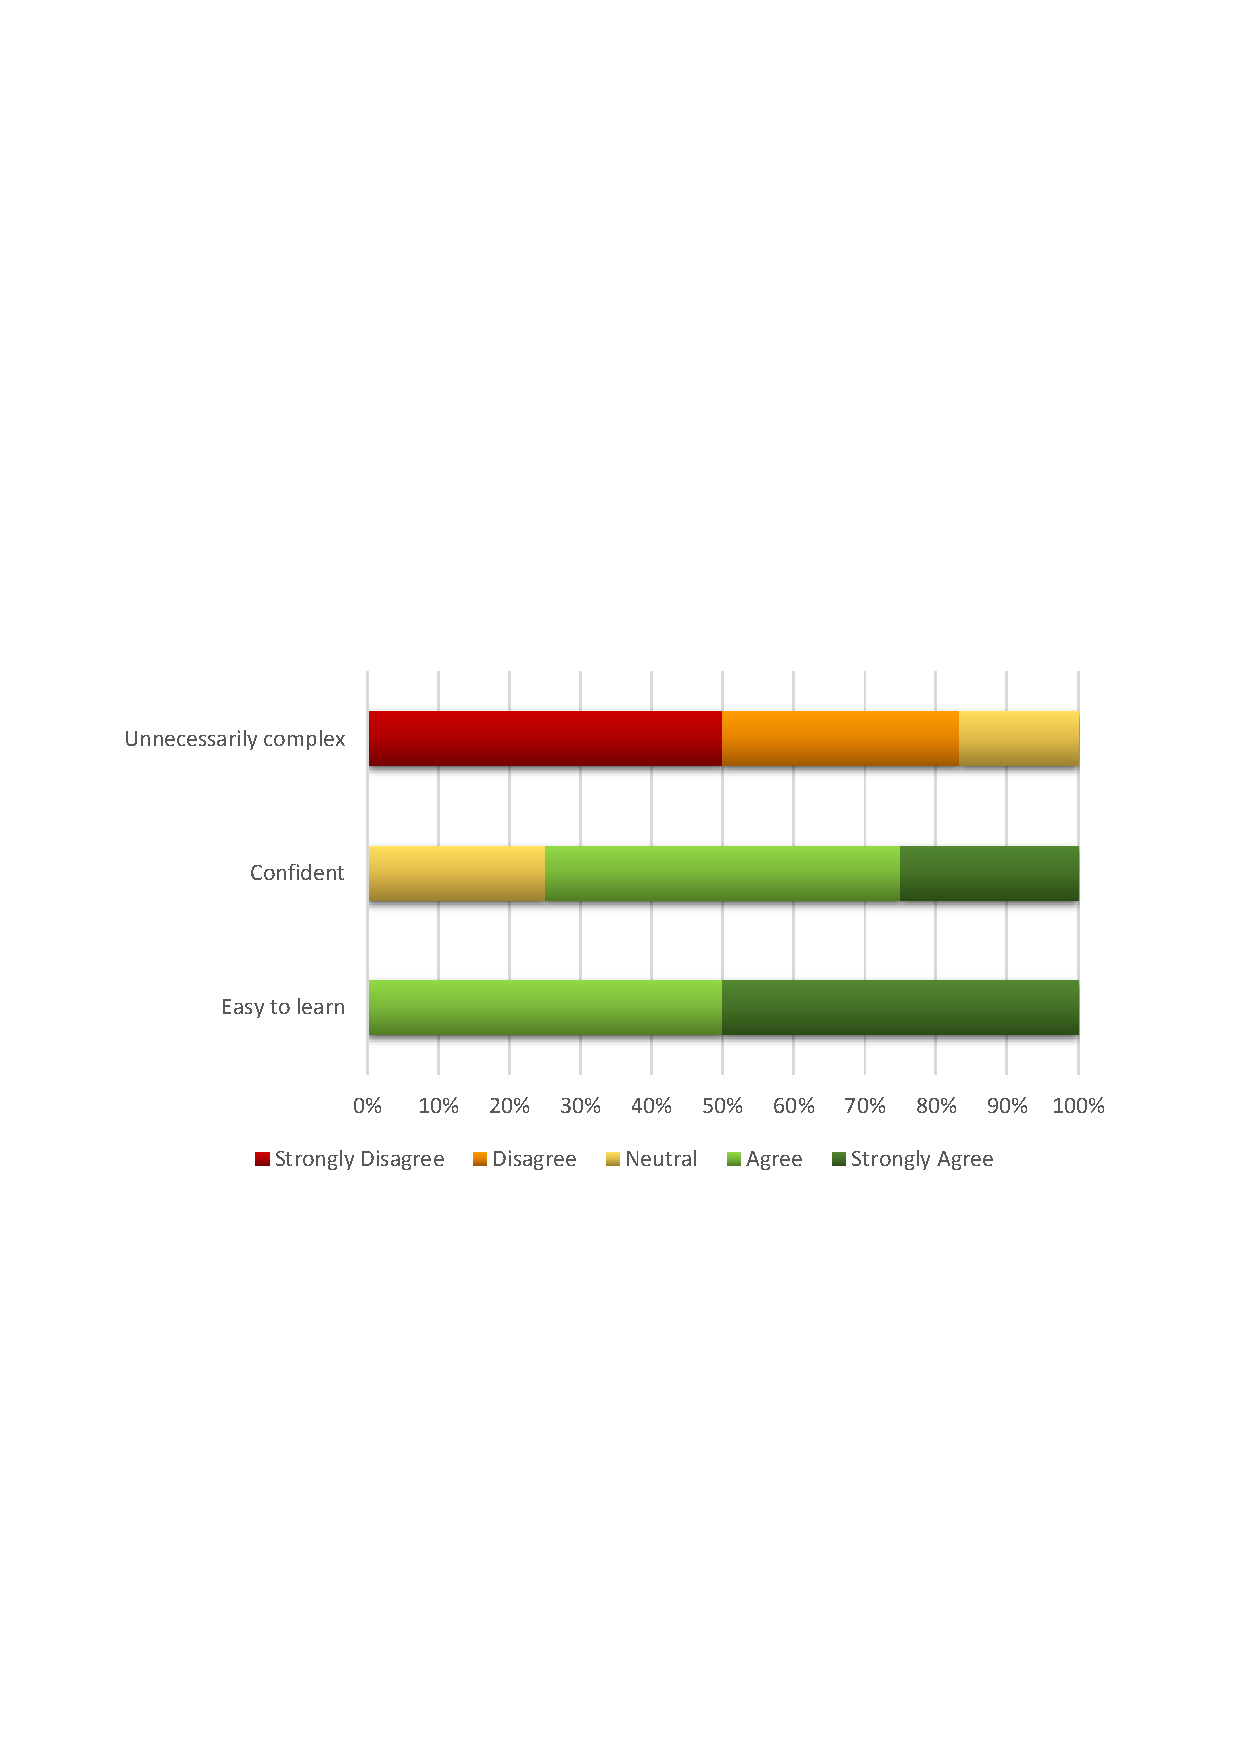
\includegraphics[width=0.8\textwidth]{images/charts/tool_general.pdf}
	\caption{General evaluation of our tools}
	\label{fig:tool_general}
\end{figure}

Figure ~\ref{fig:would_use_features} shows which features the participants would use for implementing and debugging cross-device applications. In general, people would rather use emulated devices than connecting real devices for both implementing and debugging. This is understandable as most things can be done just as well with emulated devices as with real devices. Some participants mentioned that they would not really use real devices during implementing, but that they would test their application on real devices after finishing implementing to make sure the application works fine on them. The connection features are almost unavoidable to use, thus it is surprising that some participants state that they would not use them. However, for some parts of debugging and implementing, one device might be sufficient for testing and no connection features would be required. One participant mentioned that the connection features seem very natural and that there is no point in asking about their usefulness because it is obvious that they are useful. This indicates that the feature was indeed greatly appreciated by some participants. The shared JavaScript console is equally popular for debugging and implementing and would be used by almost all participants, thus it seems to be a very popular feature as well. Function debugging is more popular for debugging than for implementing. This corresponds to the actual results of the study and has been elaborated before. Apart from connecting real devices, the shared CSS editor is the least popular. This may be due to the fact that browsers already have quite mature CSS editors and it might be possible to test CSS on one device at a time in many cases. Also, the CSS parts of our tasks were rather simple, thus the real value of such a feature might not be obvious to the participants. While things like changing the background color of a button can easily be done on just one device, more complex CSS problems like positioning elements require more effort and look much different on different devices. Furthermore, cross-device applications do not always show the same things on all devices and applying CSS to all devices is of no use if the corresponding elements are only shown on one device anyways.

\begin{figure}[H]
  \centering
    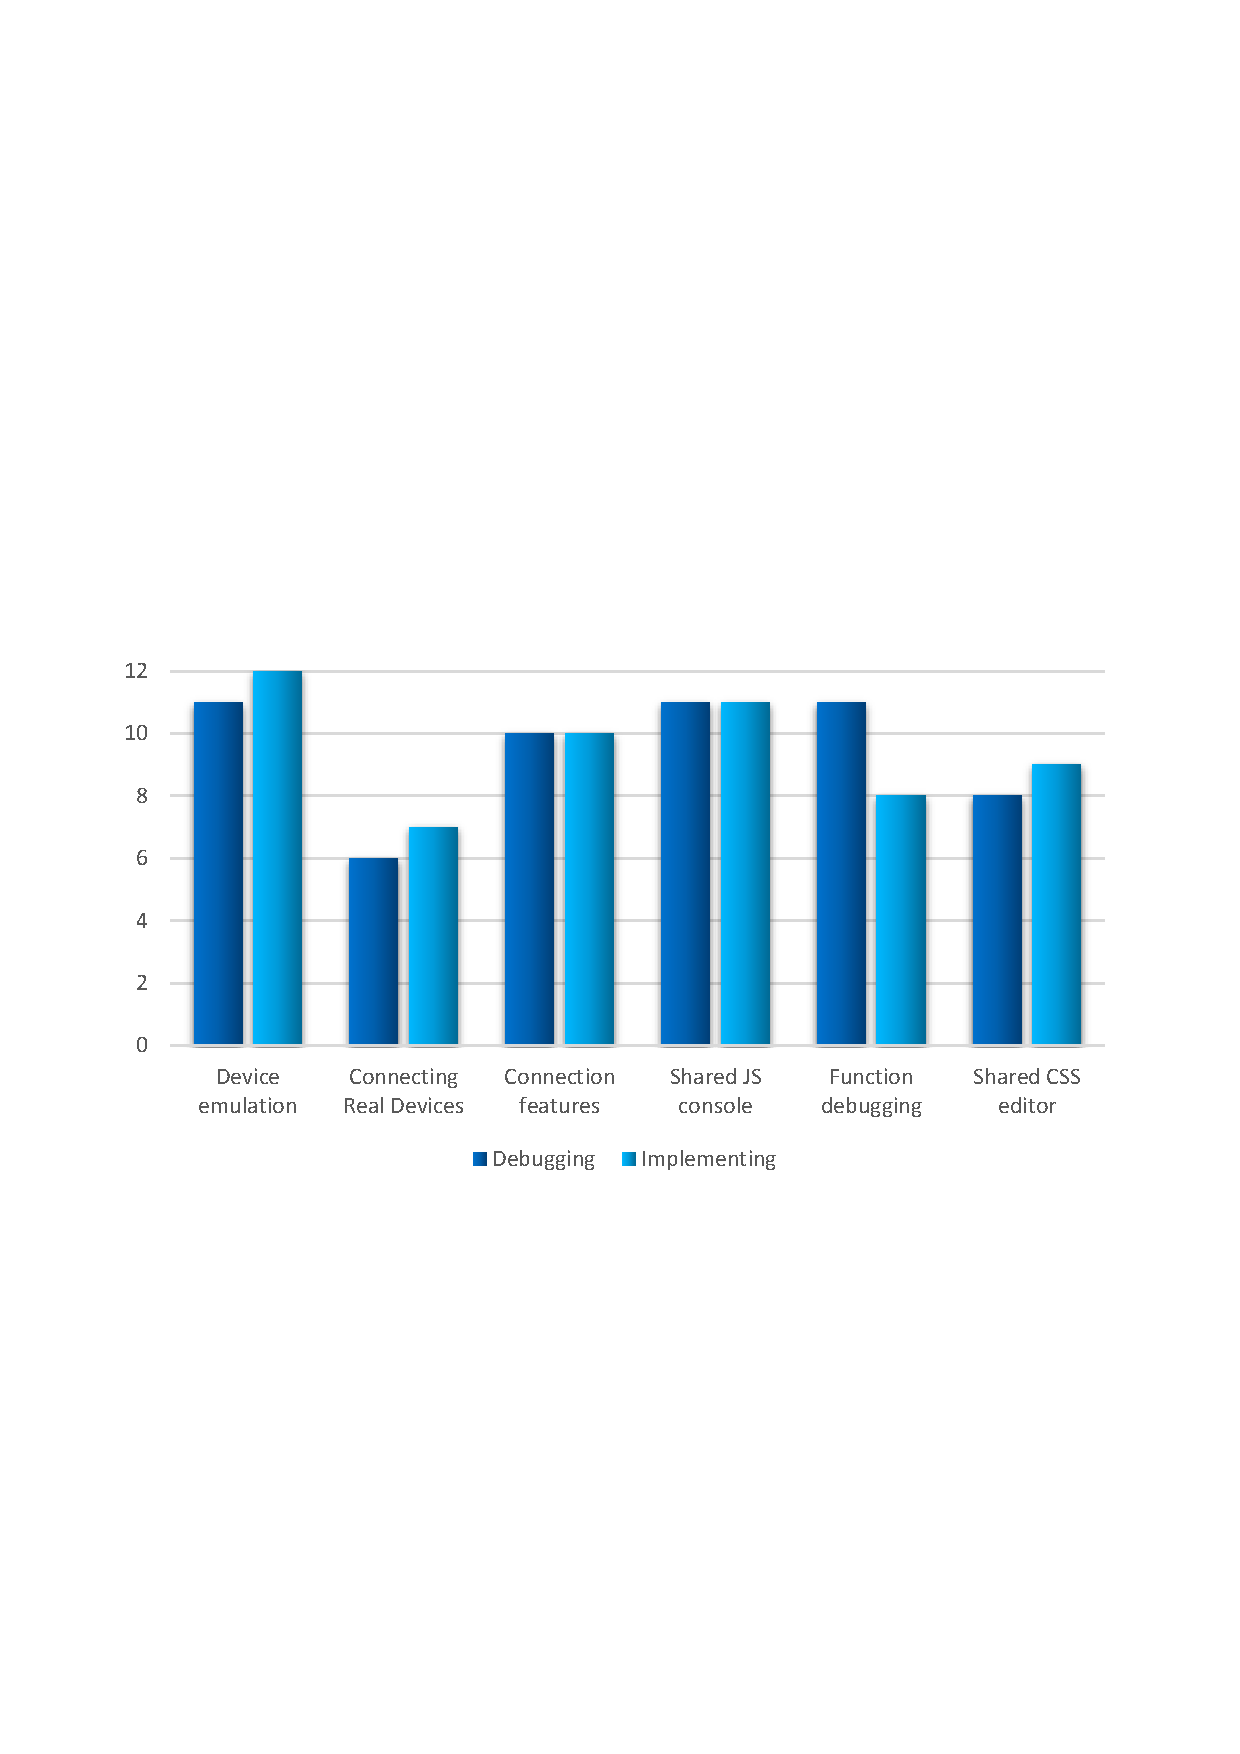
\includegraphics[width=0.8\textwidth]{images/charts/would_use_features.pdf}
	\caption{Features that the participants would use}
	\label{fig:would_use_features}
\end{figure}

During the study, some participants mentioned that they found device emulation very useful because they can have all devices in one place instead of having to manage different browser windows and profiles. Reloading all devices at once was also considered very useful. With multiple browser windows, each window has to be reloaded individually which makes this a much more tedious task. It was also appreciated that the devices are still connected after reloading, though this is also the case with multiple browser windows. The participants really liked function debugging, the only critique was that it does not show on which device a function is called which was fixed after the study. In general, the output aggregation of the shared JavaScript console was considered more useful than sending commands. One participant even mentioned that he would not use it to send commands, but the aggregation is very useful. 

In general, the feedback during the study showed that participants really liked the tool. One participant stated that they think that the tool is very useful and they wish they had access to it when they were working on a cross-device application. Another participant mentioned that "The existing features are already very impressive and work well. They really help the developer working on cross-device applications."

Record/replay was disabled for the user study, but one participant that had attended a presentation about our tools before, mentioned that they would find it immensely useful. They consider it as a powerful feature that could be very helpful for replicating bugs in an application and for regression testing. Often, it is not clear how to reach a bug and being able to record the set of interactions that lead to the bug and then replay them can simplify this process.

\subsubsection{Aborted Tasks}

Due to the time limits that we set, we also had to abort some tasks. There were five cases where we had to abort the task, four while participants had access to our tools, and one where the participant did not have access to our tools. There was one participant that finished all task except the XDCinema debugging task. The participant had access to our tools for this task, but we do not consider this relevant for this specific case, as the time required for completing this task can vary greatly depending on how fast the participant notices the switched variable. Also, the participant had completed all other task successfully. Furthermore, there was one participant for whom we had to abort both implementation tasks (one with our tools and one without) and one participant where we had to abort both XDCinema tasks (both with our tools). Both those participants had very low experience in web application development and had problems completing basic things like placing brackets correctly around an if-statement and creating a new line in HTML. This indicates that those participants had very low programming experience in general and it is not surprising that they failed to complete some tasks. The participants also had problems completing the other tasks, but eventually managed to finish the tasks with a lot of help from the instructor. Thus, we do not think that the fact that most of the aborted tasks were carried out with our tools says anything relevant about our tools. It was simply bad luck that most of the aborted tasks were carried out in this condition.

\subsubsection{Devices Used}

Overall, the number of devices used did not vary greatly depending on the participant and on the condition the participant was in. Although our tasks were designed to require at least two devices in general, it was possible to complete the XDCinema debugging task with only one device, but the task required less device interaction when multiple devices were involved. Figure ~\ref{fig:n_emulated} shows how many emulated devices the participants used on average with and without our tools. The number of emulated devices used is slightly higher with our tools for all tasks. One reason for this difference could be that it is easier to add a new device with our tools. However, the difference is rather small and further investigation is needed to see if this is really the case. For the XDCinema debugging task, only two out of six participants that did not have access to our tools used more than one device. With our tools, four participants used more than one device. This also indicates that participants prefer to use more devices when they have access to our tools. For the XDCinema implementation task, all participant used exactly three devices (when combining real and emulated devices) which is not surprising because the minimum number of devices required was three and additional devices did not provide any value. 

\begin{figure}[H]
  \centering
    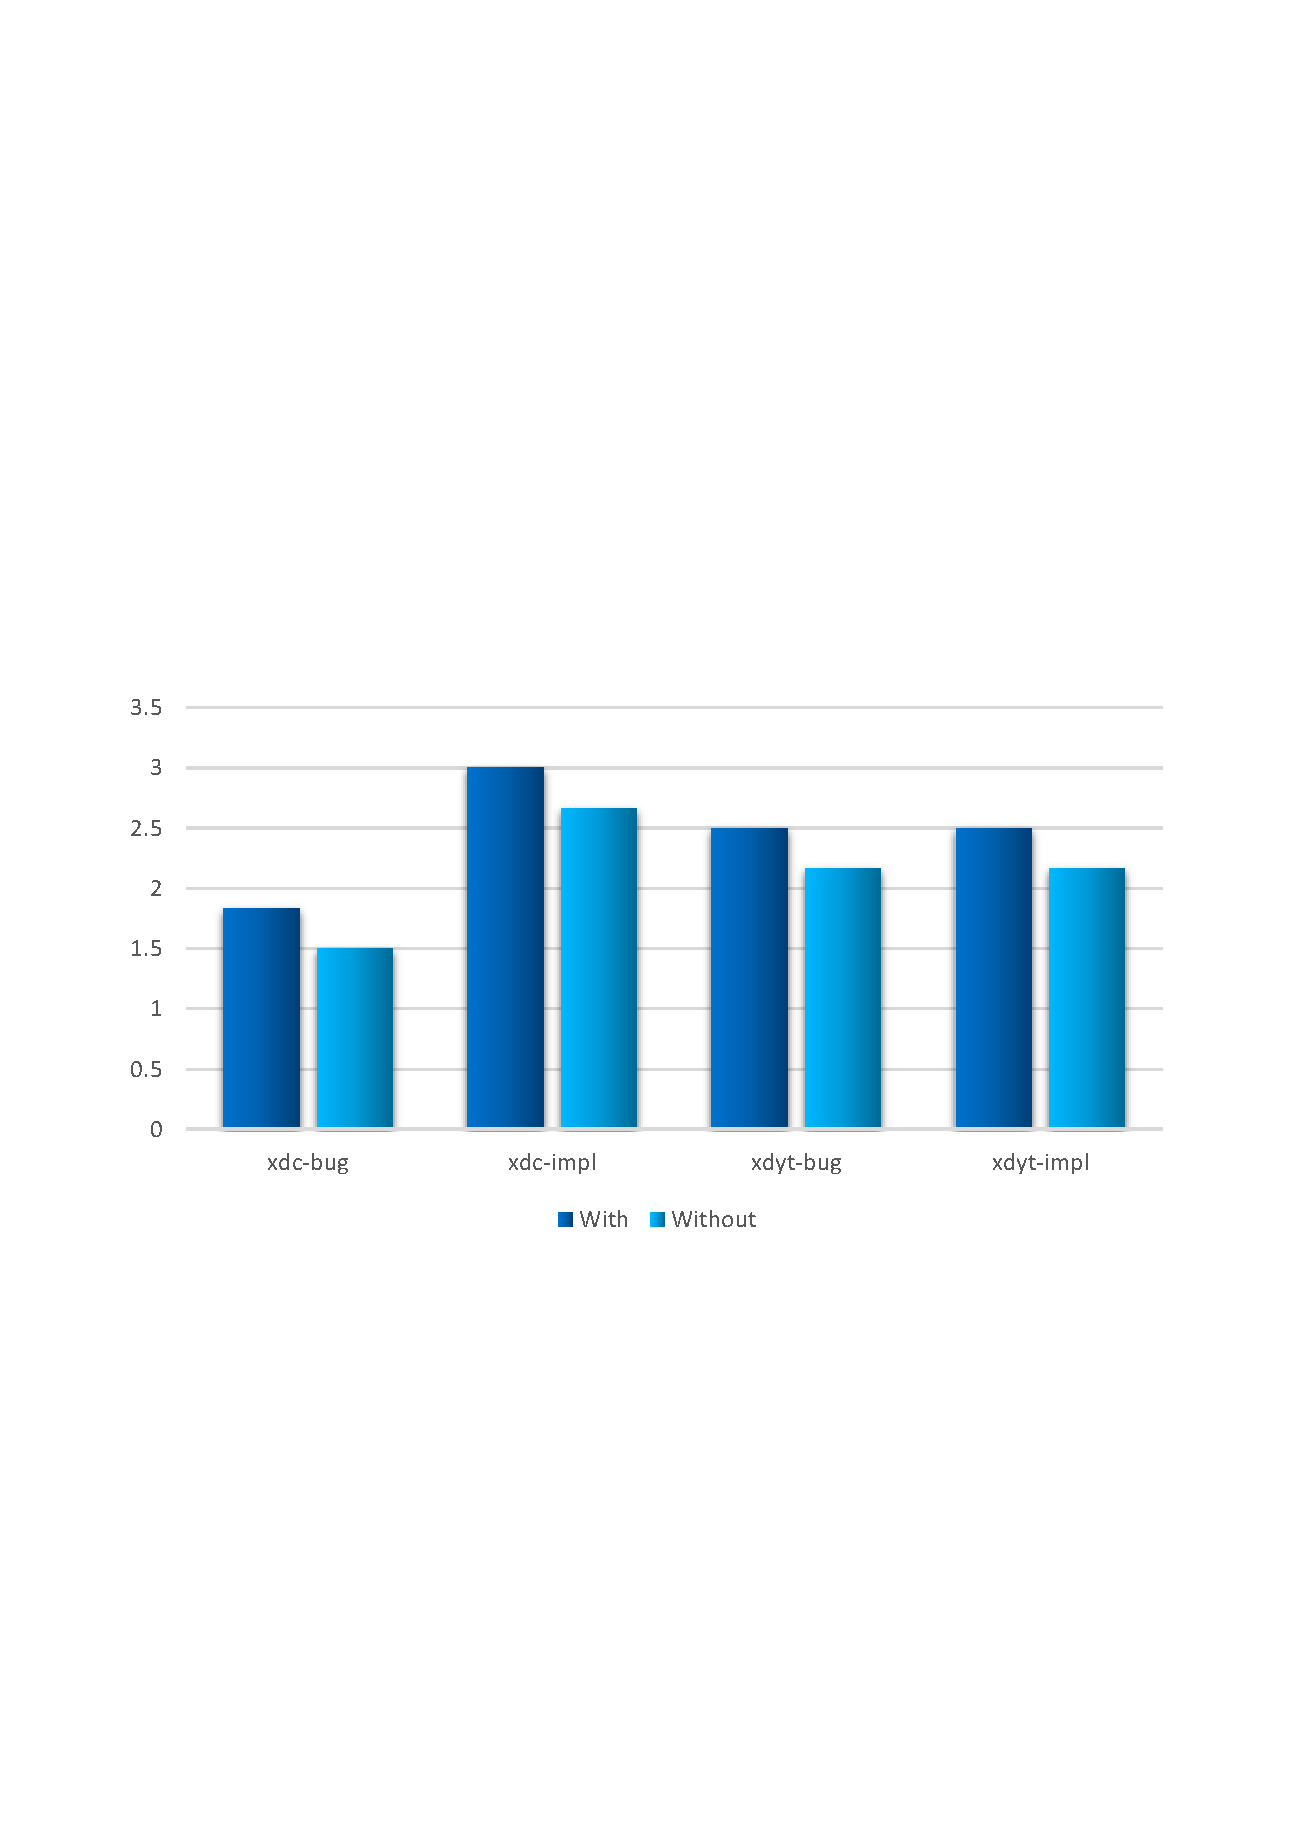
\includegraphics[width=0.8\textwidth]{images/charts/n_emulated.pdf}
	\caption{Average number of emulated devices used}
	\label{fig:n_emulated}
\end{figure}

The real devices were only rarely used overall. In the XDYouTube implementation and debugging tasks, one participant per condition used one real device. In the XDCinema implementation task, one participant that did not have access to our tools used two real devices, further supporting our thesis that adding emulated devices is more tedious without access to our tools. Normally, most of the tasks required for implementing cross-device applications can be performed just as well on emulated devices. Testing on real devices is typically limited to points where major implementation steps have been completed or when a developer wants to see how interactions feel or work on actual touch devices. Therefore, it is no surprise that real devices were not used frequently during our study. The number of devices used during the tasks shows that although participants sometimes stick to the minimum number of devices required, they also like to be able to add more devices for convenience of further testing. In the XDYouTube implementation task, participants often added three devices so they could put one in landscape mode and one in portrait mode. This allowed them to add videos to the queue and test their implementation of the remote control button without switching orientation in-between. 

In terms of screen sizes used, participants mostly used low-resolution mobile phones and sometimes tablets when carrying out tasks with our tools. The devices were in portrait mode at almost all times, except for when they were required to be in landscape mode by the application. This is probably due to the dimensions of the area where devices can be placed which makes it more convenient to have devices in portrait mode. Furthermore, most predefined devices are in portrait mode by default and participants did not switch their orientation unless required to. Without access to our tools, participants also often used smaller devices, but sometimes they had one large full-screen browser window and other smaller browser windows that they just switched to when required. Participants that used three devices often let one device fill the left half of the screen and let the other two devices fill one quarter of the screen each, which put them in landscape mode. 

\subsubsection{Debugging/Implementation Strategies}

In both debugging tasks and both conditions, about half the participants started by looking at the code and about half started by trying to reproduce the bug. Most of the participants switched between the code and the application multiple times while carrying out the tasks, although some looked at the code directly in the DevTools. Almost all participants used the DevTools at some point for completing the task, and most of the participants that had access to our tools used function debugging. The debugging task in XDCinema and XDYouTube had some fundamental differences: The main difficulty for the XDYouTube debugging task was reproducing the bug, once the bug was reproduced, the cause of the bug was pretty obvious given the JavaScript error the bug produced. In contrast, reproducing the bug in the XDCinema debugging task was trivial, but finding out what causes the bug is more difficult. In XDYouTube, participants usually spent quite a lot of time trying to reproduce the bug before they switched to the DevTools or function debugging. Only after participants failed at reproducing the bug, they used tools for debugging in an attempt to find the bug in this way. In XDCinema, participants switched to the DevTools or function debugging much faster because they reproduced the bug almost immediately. Consequently, in XDYouTube, much more time is spent switching between the code and application because the participants try out different ways of finding the bug. In XDCinema, the debugging process is much more streamlined because after reproducing the bug, participants mostly stick to either looking at the code or using tools for debugging.

In the implementation task, some participants started by looking for the HTML-element that contained the prices or the remote control button first, while others started implementing right away. All participants implemented everything required for the XDYouTube implementation task at once and only then started testing it. Only the CSS was usually added after making sure that the button works. On one hand, it makes sense to implement the complete remote control functionality at once because if only part of it was implemented, it would be difficult to see if the implemented function actually works. On the other hand, we would have expected that at least some participants implemented part of the functionality and used logging mechanisms to see if it works. In the XDCinema implementation task, the task was clearly separated into to parts and the first part did not require the second part to work. Thus, all except one participant implemented the first part, tested it, and then moved on to the second part. However, almost all participants had to modify their first part a little bit while implementing the second part because of the different requirements. The CSS part of the task was again implemented after completing everything else by most participants.

In summary, no real difference in implementation and debugging strategies can be seen between the two conditions of our study. The only difference is that some parts of the debugging process are made more efficient or easier because the developer has access to additional tools. Thus, developers should be able to use the same strategies for debugging and implementing features as they usually would and augment them with additional features where it is useful. 

\subsubsection{Feature Requests}

During the study, some participants suggested some improvements to existing features that would help them even more. Multiple participants suggested that function debugging should show on which device a function is called. We were able to successfully implement this feature after completing the user study. Also, one participant said that auto-connect should be enabled by default because there rarely is a situation where a developer would not want to connect the devices. Over the course of the study, it became obvious that this feature would be useful because many participants forgot to enable auto-connect before adding more devices and thus either manually connected them or removed them, enabled auto-connect, and re-added the devices. Furthermore, it was suggested that the border of the device should be in the device's unique color so devices can more easily be recognized. Those two features were also included into our tools after the study. Also, it became clear during the study that it was not at all obvious when function debugging was working and when the participants had to re-open the DevTools. Due to this, we now show a warning when the developer should re-open the DevTools to make sure that function debugging works. Also, we now display a warning message when the user wants to reload the page because many participants accidentally reload the page instead of the devices and then lose all their devices. Some additional feature suggestions include:
\begin{itemize}
	\item CSS value suggestions, e.g. suggest "1px solid black" when the developer sets the border property
	\item More integration with the DevTools
	\item Opening the DevTools automatically when the developer wants to debug a function
	\item Auto-complete or similar for functions in function debugging
	\item Combining a source code editor with our tools
\end{itemize}
Due to time constraints and in some cases also feasibility constraints we were not able to implement those feature requests (yet). Also, while some of those requests like CSS value suggestions would clearly be useful, others like combining a source code editor with our tools require more research to determine if they are actually desired by developers and would provide some additional benefits.